% -------------------------------
% Plantilla del TFG en la ESIIAB-UCLM. Versión 0.1
%
% Luis de la Ossa
%
% Compilar con XeLaTeX
% -------------------------------
\documentclass[12pt, a4paper]{book}

% -------------------------------
% Información y opciones del documento. Debe editarse.
% -------------------------------
% -------------------------------
% Plantilla del TFG en la ESIIAB-UCLM. Versión 0.1
%
% Luis de la Ossa
%
% Compilar con XeLaTeX
% -------------------------------


% -------------------------------
% Comandos comunes
% -------------------------------
\newcommand{\uclm}{University of Castilla-La Mancha\,}
\newcommand{\dsi}{Computing Systems Department\,}
\newcommand{\esii}{School of Computer Science and Engineering\,}


% -------------------------------
% Comandos específicos
% -------------------------------
\newcommand{\autor}{Student's name\,}
\newcommand{\titulo}{Disertation title \,}
\newcommand{\director}{Supervisor's name\,}
\newcommand{\codirector}{Co Supervisor's name\,}
\newcommand{\fecha}{November, 2025\,}
\newcommand{\espec}{ Specialization\,}


% -------------------------------
% Configuración del documento, paquetes, etc.
% -------------------------------
\input{include/configuracion}

% Documento
\begin{document}

% -------------------------------
% Portada y título
% -------------------------------
% Fuente  de la portada
% Carlito = metric-compatible substitute for Calibri (original template font),
% available on Linux and CI via the ttf-carlito / fonts-crosextra-carlito package.
% \setmainfont[Ligatures={NoRequired,NoCommon,NoContextual}]{Carlito}
\input{elements/portada}

% -------------------------------
% Fuente del documento.
% -------------------------------
\setmainfont[Ligatures={NoRequired,NoCommon,NoContextual}]{Carlito}

% -------------------------------
% Preámbulo
% -------------------------------
\frontmatter
% -------------------------------
% Plantilla del TFG en la ESIIAB-UCLM. Versión 0.1 (Preliminar)
%
% Luis de la Ossa
%
% Compilar con XeLaTeX
% -------------------------------


% -------------------------------
% Segunda portada
% -------------------------------
\cleardoublepage
\setcounter{page}{1} \null


\begin{textblock*}{\textwidth}(3cm,2.4cm)
\begin{flushright}

\includegraphics[height=1.1cm]{figs/logouclm.jpg}
\end{flushright}
\end{textblock*}



\begin{textblock*}{\textwidth}(3cm,2.5cm)  % Corrige la posición porque la imagen tiene margen
\begin{flushleft}

\includegraphics[height=1cm]{figs/logoesii.png}
\end{flushleft}
\end{textblock*}



\begin{textblock*}{\textwidth}(3cm,7cm)
\begin{center}\doublespacing
{\fontsize{18pt}{4pt}\selectfont \bft{UNDERGRADUATE DISSERTATION}}

\medskip
{\fontsize{18pt}{4pt}\selectfont Bachelor's Degree in Computer Science and Engineering}

\medskip
{\fontsize{16pt}{4pt}\selectfont \espec}
\end{center}
\end{textblock*}


\begin{textblock*}{\textwidth}(3cm,13cm)
\begin{center}\doublespacing
{\fontsize{22pt}{4pt}\selectfont \bft{\titulo}}
\end{center}
\end{textblock*}


\begin{textblock*}{\textwidth}(3cm, 20cm)
\begin{flushleft}\doublespacing
{\fontsize{14pt}{4pt}\selectfont \bft{Author:} \autor}

{\fontsize{14pt}{4pt}\selectfont \bft{Supervisor:} \director}

{\fontsize{14pt}{4pt}\selectfont \bft{Co-supervisor:} \codirector}
\end{flushleft}
\end{textblock*}


\begin{textblock*}{\textwidth}(3cm,25.25cm)
\begin{flushright}
{\fontsize{14pt}{4pt}\selectfont \fecha}
\end{flushright}
\end{textblock*}


% -------------------------------
% Dedicatoria
% -------------------------------
\cleardoublepage
\thispagestyle{empty}

\vspace*{9cm}
\begin{flushright} \em
Aquí va la dedicatoria que cada cual \\
quiera escribir. El ancho se controla \\
manualmente
\end{flushright}


% -------------------------------
% Declaración de autoría
% -------------------------------
\cleardoublepage
\thispagestyle{plain}
\begin{center}
\Large{\bft{Autorship Statement}}
\end{center}
\vskip1cm

I, the undersigned, \quad \ldots \quad, with ID number \quad \ldots \quad, declare that I am the sole author of the Undergraduate Dissertation titled ``\quad \ldots \quad '', that this work does not break the current intellectual property law. and that all the non-original material contained in this work is properly attributed to their legitimate authors.

\vspace*{2cm}
\begin{center}
Albacete, (date)

\vskip3cm

Signed by: \autor
\end{center}


% -------------------------------
% Resumen
% -------------------------------
\cleardoublepage
\thispagestyle{plain}
\begin{center}
\Large{\bft{Abstract}}
\end{center}
\vskip1cm

\lipsum[1]

% -------------------------------
% Agradecimientos
% -------------------------------
\cleardoublepage
\thispagestyle{plain}
\begin{center}
\Large{\bft{Acknowledgements}}
\end{center}
\vskip1cm

\lipsum[1]


% -------------------------------
% Índices y tablas
% -------------------------------
% Cambia a interlineado normal
\singlespacing

\tableofcontents	% Índice
\listoffigures		% Índice de figuras
\listoftables		% Índice de tablas
%\listofalgorithms   % Índice de algoritmos (comentar si no los hay)
%\listofcodes	    % Índice de códigos (comentar si no los hay)
\cleardoublepage

% Vuelve a interlineado de 1.5
\onehalfspacing

% -------------------------------
% Documento
% -------------------------------
\mainmatter
% Estilo de página
\pagestyle{fancy}


% Introducción
\chapter{Introduction}
\label{ch:intro}

% Allow a little extra line stretch so long technical compounds rebreak
% cleanly instead of spilling into the margin (no template packages added).
\setlength{\emergencystretch}{3em}

\section{Introduction}
\label{sec:intro-context}

Over the last two decades almost every activity of economic or social consequence
has moved onto networked software. Commerce, banking, public administration,
healthcare, industrial control and private communication are now mediated by web
applications, mobile clients and the programming interfaces that join them: a
business that once required a physical counter is today a service reachable from
anywhere. That migration has been accompanied by an accumulation of data without
precedent. Identity documents, payment instruments, clinical histories, location
traces and corporate intellectual property all sit in systems that are, by design,
reachable over a public network. Data of this kind is no longer a by-product of
doing business; it is an asset in its own right, and frequently the most valuable
one an organisation holds.

Anything valuable attracts people who want to take it, and their motives are as
varied as the data itself. Some adversaries pursue direct financial gain, through
fraud, payment-card theft or the resale of credentials on criminal markets. Others
pursue extortion, encrypting or exfiltrating an organisation's own data and charging
for its return. Others act on behalf of states, for espionage, sabotage or
geopolitical advantage, targeting infrastructure and industry rather than
individuals. What they share is the route in: a flaw in the software, or in the way
it was configured, that permits something its designer never intended.

Guarding against them is the business of cybersecurity, and doing so credibly takes
more than good intentions at design time. Security is not a property an organisation
can assert about itself; it is one that must be demonstrated against an adversary
actively looking for the exception. This is the purpose of the security audit and,
in particular, of the \emph{penetration test}: a controlled, authorised exercise in
which a professional attacks a system as a real adversary would, to establish
empirically what an attacker could achieve and how mature the defences actually are.
The practice is established enough to be codified in methodologies and standards
such as the PTES, the OWASP Web Security Testing Guide, the OSSTMM and NIST
SP~800-115 \cite{ptes, owasp_wstg, osstmm, nist80015}, and in regulated sectors it
is mandated outright: PCI~DSS requires not only that penetration testing be
performed, but that the weaknesses it finds be corrected \emph{and the testing
repeated to verify the correction} \cite{pcidss}.

That final clause is where the practice meets a problem, and it is the problem this
dissertation addresses. An audit creates value only if its findings are fixed, and a
fix counts only once somebody confirms it. This confirmation step, the
\emph{revalidation} or retest of reported findings, is routine, repetitive and
poorly automated. A security audit ends with a report listing each discovered
vulnerability and the steps needed to reproduce it; once the development team applies
fixes, someone must verify that those fixes actually work, that each finding is
genuinely closed rather than incidentally hidden. The stakes are not academic. Known,
previously identified vulnerabilities that are never properly closed remain a leading
cause of breaches: in a survey of nearly 3{,}000 practitioners, 60\% of breach victims
traced their compromise to a known vulnerability whose patch was available but had not
been applied \cite{ponemon_vulnerability_2019}. Yet this re-testing is still performed
largely by hand, one finding at a time, on every remediation cycle, and it demands
careful judgement to avoid declaring a still-exploitable weakness ``fixed''. It is
exactly the kind of high-volume, judgement-laden, evidence-driven task at which a
well-supervised AI assistant should be able to help. The manual character of
revalidation is examined in detail in Section~\ref{subsec:revalidation}.

Artificial intelligence, meanwhile, is advancing faster than almost any previous computing
technology, and the capabilities of the underlying models are improving on a
timescale measured in months rather than years. Each new generation of large
language model is not only more fluent but more \emph{autonomous}: able to plan,
use tools, write and debug code, and pursue a goal across many steps with little
human direction. Cybersecurity sits squarely in the path of this progress,
because the same reasoning-and-acting ability that makes a model a capable
programming assistant also makes it a capable attacker. Keeping pace with this
acceleration is no longer optional for the defensive side; it is a precondition
for staying relevant.

The offensive use of this technology is already a documented reality rather than
speculation. Purpose-built ``dark'' language models such as WormGPT and FraudGPT,
sold on underground forums as safety-stripped alternatives to mainstream
assistants, lower the barrier to entry for phishing, malware generation and social
engineering \cite{malla2024}. State-affiliated threat actors from several countries
have been observed using mainstream models for reconnaissance, scripting and
translation in support of their operations \cite{openai_threatactors}. Research has
shown that autonomous agents can exploit real vulnerabilities directly from their
public descriptions, with no prior knowledge of the flaw \cite{fang2024oneday}. In
November 2025 this trajectory reached a milestone: the first publicly reported
cyber-espionage campaign in which an AI agent executed the large majority of the
intrusion (reconnaissance, exploitation, credential harvesting and lateral
movement) with only sporadic human oversight \cite{anthropic_espionage}.

The frontier has moved further still. In April 2026 Anthropic previewed
\emph{Mythos}, a model whose cybersecurity capability, described as an emergent
side-effect of broader gains in reasoning and autonomy, proved strong enough that
the company declined to release it openly \cite{anthropic_mythos}. Operating with
little human steering, Mythos discovered thousands of high- and critical-severity
vulnerabilities across widely used software and produced working exploits in hours
for flaws that had survived decades of human review, including long-dormant bugs in
mature, security-focused systems; an independent assessment by the United Kingdom's
AI Security Institute corroborated the scale of these results
\cite{aisi_mythos}. Nor is such capability confined to frontier laboratories: the
autonomous penetration-testing system XBOW climbed to the top of a major public
bug-bounty leaderboard, out-reporting human researchers over a sustained period
\cite{xbow}. The economics are shifting decisively: work that took expert teams
weeks can increasingly be attempted overnight. Figure~\ref{fig:timeline} places
these milestones on a single timeline; barely three years separate the first
commodity malicious chatbot from autonomous exploitation at the frontier.

\begin{figure}[htbp]
\centering
\begin{tikzpicture}[
  >={Stealth[length=2mm]},
  ev/.style={rounded corners=2pt, align=center, inner sep=3pt, text width=2.7cm, font=\scriptsize},
  off/.style={ev, draw=rojo, thick, fill=rojo!6},
  def/.style={ev, draw=azul, thick, fill=azul!6},
]
\draw[->, thick, gris50] (-0.5,0) -- (14.4,0);
\foreach \x/\yr in {1/2023, 5/2024, 9/2025, 13/2026} {
  \draw[gris50, thick] (\x,0.12) -- (\x,-0.12);
  \node[font=\footnotesize\bfseries, text=gris25] at (\x,-0.42) {\yr};
}
\node[off, anchor=south] (worm)   at (1,0.55)  {WormGPT / FraudGPT malicious LLMs};
\node[off, anchor=south] (nation) at (5,0.55)  {Nation-state LLM misuse};
\node[off, anchor=south] (xbow)   at (9,0.55)  {XBOW tops bug-bounty leaderboard};
\node[off, anchor=south] (mythos) at (13,0.55) {\emph{Mythos}: autonomous discovery + exploitation};
\node[def, anchor=north] (bigsleep) at (5,-0.7)  {Big Sleep finds real-world 0-day};
\node[off, anchor=north] (esp)      at (9,-0.7)  {First AI-orchestrated espionage campaign};
\draw[gris50] (1,0)  -- (worm.south);
\draw[gris50] (5,0)  -- (nation.south);
\draw[gris50] (9,0)  -- (xbow.south);
\draw[gris50] (13,0) -- (mythos.south);
\draw[gris50] (5,0)  -- (bigsleep.north);
\draw[gris50] (9,0)  -- (esp.north);
\end{tikzpicture}
\caption[Timeline of the offensive-AI arms race]{Selected milestones in the use of artificial intelligence for cyber-offence (red) and cyber-defence (blue), 2023--2026.}
\label{fig:timeline}
\end{figure}

Defenders are not without their own AI. The same class of models has been turned to
protective ends: Google's Big Sleep agent autonomously found a previously unknown
vulnerability in production software and later helped pre-empt one that attackers
were preparing to use \cite{google_bigsleep}. The difficulty is one of balance.
Offensive capability scales cheaply and runs unattended, whereas much defensive
work remains gated by manual, human-paced procedures. Where the two sides draw on
the same technology, the advantage accrues to whoever removes the human bottleneck
first, and, on the defensive side, many of the most important bottlenecks have
not yet been addressed.

These two threads meet at the revalidation problem. One side of the audit cycle,
the attack, is being automated at remarkable speed; the other, the confirmation that
what the attack found has genuinely been fixed, is still done by hand. This
dissertation proposes to close part of that distance with a tool, named
\emph{revalid}, that applies an AI agent to the revalidation of reported findings:
it reads a penetration-test report, interprets each finding's reproduction steps,
and re-executes them against an authorised target under human supervision, returning
an evidence-backed verdict on whether the finding is closed. The remainder of this
chapter states why the work was undertaken, what it set out to achieve, and how the
document is arranged.

\section{Motivation}
\label{sec:motivation}

Two motivations, one personal and one technical, brought this project about.

The personal one came first. Artificial intelligence applied to cybersecurity is the
area of the discipline I find most compelling, and the one I intend to keep building a
career in. A final-year project is a rare opportunity to work on a problem at that
intersection with enough depth to actually learn the craft rather than sample it, and
to do so across the whole lifecycle of a system: designing it, building it, evaluating
it honestly and writing it up. Choosing a subject that sits squarely between offensive
security and applied AI was therefore a deliberate investment in a direction I want to
keep growing in, and much of what the work taught is reported in
Section~\ref{sec:lessons}.

The technical motivation is the gap the first one led me to. Revalidation is not
unautomated: pentest-management platforms track it as a workflow, and automated
security-validation products genuinely re-run their checks after a fix. But those two
capabilities sit on opposite sides of a line. The platforms that are driven by the
content of a report hand the actual verification to a human, while the products that
automate verification re-run only the findings \emph{they themselves} discovered, from
their own internal model of the target, and cannot take in a report written by an
external auditor. Nothing surveyed in Section~\ref{sec:sota} occupies the intersection:
re-executing the reproduction steps of a specific, externally reported finding and
returning a per-finding verdict on it. That gap is narrow, and closing it is worth
doing precisely because the case it leaves uncovered, an audit performed by someone
else, is the ordinary one for most organisations.

\section{Goal and objectives}
\label{sec:objectives}

The goal of this project is to advance the defensive side of this arms race by
giving security professionals, the cybersecurity architects, auditors and
developers responsible for closing the loop on an audit, an AI-driven tool that
accelerates the revalidation of vulnerabilities through \emph{assistance} rather
than replacement. Concretely, the general objective is:

\begin{quote}
\emph{To automate the retesting of reported vulnerabilities using artificial
intelligence, in order to reduce response time and increase efficiency in security
audits, while keeping a human in control of every action that touches a target.}
\end{quote}

This general objective is refined into four specific objectives, which structure the
work reported in the remaining chapters:

\begin{enumerate}[labelindent=\parindent, leftmargin=*, label=\mbox{\bft{[O\arabic*]}}]
\item \bft{Analyse and structure penetration-test reports}, identifying for each
  finding the elements relevant to its revalidation: description, impact, attack
  vector, affected endpoints and, above all, the ordered steps needed to reproduce
  it.
\item \bft{Interpret reproduction steps into executable actions}, designing an
  AI-based component able to turn the natural-language description of a finding into
  concrete, non-destructive verification commands.
\item \bft{Develop an automated, human-supervised retesting system} that executes
  those verification actions against authorised targets and produces an
  evidence-backed verdict of \emph{still-open}, \emph{fixed} or
  \emph{inconclusive} for each finding.
\item \bft{Evaluate the accuracy and usefulness of the system}, comparing its
  verdicts against ground truth and against the effort of traditional manual
  revalidation, in terms of reliability and time saved.
\end{enumerate}

The shape of that autonomy deserves stating precisely, since O3 is worded around it. The
retest is run by the agent: it reads the finding, composes each verification command,
interprets what comes back and decides what to try next, across as many steps as the
problem takes. What the operator holds is not the work but the \emph{authority} --- each
command is authorised before it touches the target, and the operator may steer the agent,
run a command themselves or end the session at any point.
Section~\ref{subsec:llm-safety} sets out why a wholly unsupervised language-model agent
is the wrong instrument for a verdict that a compliance process will rely on, since
hallucination and over-confident conclusions are not incidental defects of these systems
but documented properties of them, and Section~\ref{sec:design-retest} shows what the
gate buys. The obvious objection is that oversight must cost speed.
Section~\ref{sec:eval-time} measures it, by running the same findings on the same backend
with the gate and without it: the difference was under three minutes in thirty, because
what a retest costs is the model's per-step latency rather than the human round-trip. A
fully unattended mode exists as well and was measured; supervision is the default, not
the only option.

\section{Proposed solution}
\label{sec:solution}

The system developed to meet these objectives, named \emph{revalid}, is a local,
single-operator web application that ingests a penetration-test report, uses a
language model to extract each finding together with its reproduction steps, and
then runs an interactive, sandboxed agent that re-verifies the finding against an
authorised lab target. Three principles distinguish it from the offensive tools
surveyed above, and from the automation reviewed in
Chapter~\ref{ch:sota}. It is \emph{report-driven}: it re-executes the reproduction
steps of a specific, human-reported finding rather than hunting for new
vulnerabilities. It is \emph{human-gated}: the agent proposes each command and a
human operator approves it before it runs, so autonomy is used to accelerate the
expert, never to remove them. And it is \emph{verdict-oriented}: its output is a
conservative, evidence-linked determination that a compliance decision can rely on,
biased toward \emph{inconclusive} whenever the evidence is ambiguous. The precise
gap this design fills is argued in Section~\ref{sec:gap}. Figure~\ref{fig:concept}
shows the pipeline at a glance.

\begin{figure}[htbp]
\centering
\resizebox{\textwidth}{!}{%
\begin{tikzpicture}[
  >={Stealth[length=2.6mm]},
  st/.style={draw=gris50, thick, rounded corners, align=center, text width=2.5cm, minimum height=1.5cm, fill=gris95, font=\scriptsize, inner sep=3pt},
  hl/.style={st, draw=rojo, very thick, fill=rojo!8},
]
\node[st] (rep) at (0,0)       {\bft{Report}\\PDF / JSON};
\node[st] (ext) at (3.2,0)     {\bft{Extract}\\findings + reproduction steps (LLM)};
\node[st] (goal) at (6.4,0)    {\bft{Goal}\\retest objective};
\node[hl] (retest) at (9.6,0)  {\bft{Gated retest}\\agent proposes, operator approves each command (sandbox)};
\node[st] (verdict) at (12.8,0){\bft{Verdict}\\still-open / fixed / inconclusive, with evidence};
\foreach \a/\b in {rep/ext, ext/goal, goal/retest, retest/verdict} {\draw[->, gris50, thick] (\a) -- (\b);}
\end{tikzpicture}%
}
\caption[What \emph{revalid} does]{The \emph{revalid} pipeline, from report to evidence-backed verdict. The gated retest, where human control is exercised, is highlighted.}
\label{fig:concept}
\end{figure}

\section{Development methodology}
\label{sec:methodology}

The project was developed as an individual software-engineering effort following a
lightweight, Kanban-based iterative process, with every functional requirement
tracked as an issue on a project board and integrated through a
continuous-integration gate before merging. Design decisions of any significance
were recorded as architecture decision records, and the software is covered by an
automated test suite across unit, integration and system levels. In keeping with
the pace of the technology it studies, the project itself was built with the
assistance of AI coding tools under human review; the nature and extent of that
assistance is declared, as the regulations require, in Chapter~\ref{ch:methodology}.

\section{Structure of this document}
\label{sec:structure}

The remainder of this dissertation is organised as follows.
Chapter~\ref{ch:sota} sets out the technical background, surveying penetration testing
and the vulnerability-management lifecycle, the successive waves of automation
applied to security testing, the language-model agents that now drive offensive
security, and the extraction of structured information from reports; it then reviews
the state of the art in the tools that revalidate findings today, and closes by
identifying the research gap that \emph{revalid} fills. Chapter~\ref{ch:methodology}
then sets out the methodology followed to build the system: the design-led,
AI-assisted development model, the software process adopted, the technologies used,
and the declaration of AI-tool use required by the regulation.
Chapter~\ref{ch:design} then presents the design of the system itself: the
requirements it answers to, its container and module structure, the containment
topology that enforces its safety constraints, its class and persistence models, how
it reads a report into structured findings, the gated agentic retest loop at its
centre, and the earlier architecture that was built and then deleted.
Chapter~\ref{ch:evaluation} then reports an evaluation of the system
against a real penetration-test report on a live target: the reliability of its
verdicts, and the effort it saves over manual retesting. Chapter~\ref{ch:conclusions},
finally, draws together what the work achieved and what it taught, and sets out the
directions it opens, chief among them a larger-scale evaluation building on the
one reported here. Finally, Appendix~\ref{ch:annex-install} provides a step-by-step
guide to installing and operating the system.


% Estado del arte
\chapter{State of the Art}
\label{ch:sota}

% Allow a little extra line stretch so long technical compounds rebreak
% cleanly instead of spilling into the margin (no template packages added).
\setlength{\emergencystretch}{3em}

The problem addressed by this dissertation --- deciding, after a remediation
cycle, whether a previously reported vulnerability is still exploitable --- sits at
the meeting point of two bodies of work that have grown steadily closer over the
past few years: the practice of penetration testing and vulnerability management,
and the automation of security assessment, increasingly driven by artificial
intelligence. These are not separate worlds. A sustained research and industry
effort has been pushing automation ever deeper into the security lifecycle, and the
line between a manual audit and an automated one is dissolving quickly: the very
period that produced autonomous offensive agents also produced defensive
counterparts such as Google DeepMind's \emph{CodeMender}, an AI agent that patches
newly discovered vulnerabilities and proactively rewrites existing source code to
remove whole classes of weakness, with every patch reviewed by a human before it is
upstreamed \cite{codemender}. Against this fast-moving and increasingly crowded
backdrop, the report-driven revalidation of a specific reported finding --- re-running
its own documented reproduction steps rather than a generic attack library --- is one of
the tasks this wave of automation has so far largely passed over, and it is that
omission this chapter builds toward. It first frames the manual, repetitive nature of the
\emph{revalidation} (retest) phase within the vulnerability management lifecycle
(Section~\ref{sec:pentest-lifecycle}). It then surveys the successive waves of
automation applied to security testing, from signature-based scanners to
learning-based autonomous agents (Section~\ref{sec:automation}). The following
two sections concentrate on the technology that makes this work possible: large
language models (LLMs) and the tool-using agents built on top of them
(Section~\ref{sec:llm-agents}), and the extraction of structured information from
the unstructured prose of security reports (Section~\ref{sec:ie}). The chapter
closes with a synthesis that positions the proposed system against related work
and identifies the narrow gap it targets (Section~\ref{sec:gap}).

\section{Penetration testing and the vulnerability management lifecycle}
\label{sec:pentest-lifecycle}

A penetration test is an authorised, goal-directed simulation of an attack whose
purpose is to discover and demonstrate exploitable weaknesses in a system before a
real adversary does \cite{nist80015}. Its output is a report: a structured
account of each finding, its severity, its impact, and the concrete steps needed
to reproduce it. That report is not an end in itself but the entry point to the
\emph{vulnerability management lifecycle} --- the cyclical process of
identifying, prioritising, remediating and \emph{re-verifying}
weaknesses. This section reviews the methodologies that standardise the practice,
isolates the revalidation phase that this dissertation targets, and summarises the
taxonomies used to classify and score the findings that flow through the cycle.

\subsection{Methodologies and standards}
\label{subsec:methodologies}

The discipline has converged on several public methodologies that prescribe how a
test should be scoped, executed and reported. The Penetration Testing Execution
Standard (PTES) \cite{ptes} defines seven phases, from pre-engagement interactions
to reporting, and is deliberately technology-agnostic. The Open Source Security
Testing Methodology Manual (OSSTMM) \cite{osstmm} emphasises measurable, repeatable
verification and introduces the notion of an operational security metric. For web
applications --- the scope of this work --- the OWASP Web Security Testing Guide
(WSTG) \cite{owasp_wstg} provides a catalogue of concrete test cases organised by
vulnerability class. At the institutional level, the NIST Technical Guide to
Information Security Testing and Assessment (SP~800-115) \cite{nist80015} frames
testing within a broader assessment programme and explicitly includes
\emph{re-testing} of remediated findings as part of the assessment rather than an
optional afterthought.

A common thread runs through all four documents: each treats the test as a
\emph{process} that produces evidence, and each assumes that remediation will be
followed by verification. Table~\ref{tab:standards} summarises how the principal
methodologies position the revalidation step. The recurring observation is that,
although every standard expects re-verification, none prescribes \emph{how} it
should be automated --- the activity is described as a human responsibility, to be
repeated in full whenever a fix is deployed.

\begin{table}[htbp]
\footnotesize
\renewcommand{\arraystretch}{1.3}
\begin{center}
\begin{tabular}{|L{3.2cm}|L{4.2cm}|L{5.6cm}|}
\hline
\rowcolor{tema!10}
\bft{Methodology / standard} & \bft{Primary focus} & \bft{Treatment of the retest / revalidation phase} \\ \hline
PTES & End-to-end engagement process (7 phases) & Reporting phase expects verification of fixes; procedure left to the tester. \\ \hline
OSSTMM & Measurable, repeatable verification & Repeatability is a core principle, but retest is a manual re-run of the same checks. \\ \hline
OWASP WSTG & Web-application test cases by class & Provides the concrete checks to re-run; no automation of the re-run itself. \\ \hline
NIST SP~800-115 & Institutional assessment programme & Recommends re-testing of remediated findings as part of the assessment. \\ \hline
\end{tabular}
\end{center}
\caption[Treatment of revalidation in penetration-testing standards]{How the
principal penetration-testing methodologies position the revalidation (retest)
phase. Every standard expects re-verification, yet none specifies how to
automate it.}
\label{tab:standards}
\renewcommand{\arraystretch}{1}
\end{table}

\subsection{Remediation and the revalidation phase}
\label{subsec:revalidation}

Once a report is delivered, the responsibility passes to the development or
operations team, which applies fixes and, in turn, requests confirmation that the
reported weaknesses are genuinely closed. This confirmation --- the
\emph{revalidation} or \emph{retest} --- is the phase this dissertation
automates, and Figure~\ref{fig:lifecycle} situates it within the wider
vulnerability-management cycle. It is uniquely costly for three reasons. First, it is
\emph{repetitive}: each fix triggers a re-run of the original reproduction steps,
often verbatim, against a changed system. Second, it is \emph{judgement-laden}:
deciding that a finding is fixed requires distinguishing a genuine remediation
from an incidental change --- a moved endpoint, an altered response, a disabled
feature --- that merely hides the symptom. Third, it is \emph{poorly supported by
tooling}: the report is prose, the reproduction steps are written for a human, and
no artefact links a finding to a machine-checkable verification procedure. That such
verification is necessary rather than a formality is borne out by remediation data:
across the more than five thousand penetration tests Cobalt runs each year, only
48\% of findings --- and 69\% of the most serious ones --- are ever resolved, at a
median of 67 days \cite{cobalt_pentesting_2025}; a reported fix cannot be assumed to
hold, it must be checked. Compliance regimes compound the pressure. The Payment Card Industry Data Security
Standard, for example, requires that exploitable vulnerabilities found during
penetration testing be corrected and the correction verified by repeat testing
\cite{pcidss}, turning revalidation into a recurring, deadline-bound obligation
rather than a one-off task.

\begin{figure}[htbp]
\centering
\begin{tikzpicture}[
  >={Stealth[length=2.5mm]},
  phase/.style={draw=gris50, thick, rounded corners, align=center, minimum width=3.1cm, minimum height=1.1cm, fill=gris95, font=\small},
  hl/.style={phase, draw=rojo, very thick, fill=rojo!8},
]
\node[phase] (id)  at (0,2.3) {\bft{Identify}\\\footnotesize penetration test};
\node[phase] (pr)  at (6,2.3) {\bft{Prioritise}\\\footnotesize severity (CVSS)};
\node[phase] (rem) at (6,0)   {\bft{Remediate}\\\footnotesize apply fixes};
\node[hl]    (rev) at (0,0)   {\bft{Revalidate}\\\footnotesize retest};
\draw[->, gris50, thick]    (id)  -- (pr);
\draw[->, gris50, thick]    (pr)  -- (rem);
\draw[->, gris50, thick]    (rem) -- (rev);
\draw[->, rojo, very thick] (rev) -- (id);
\node[font=\footnotesize\itshape, text=rojo, below=4pt of rev] {automated in this work};
\end{tikzpicture}
\caption[The vulnerability-management lifecycle]{The vulnerability-management
lifecycle: a finding moves from identification through prioritisation and
remediation to revalidation --- the retest that confirms the fix before the cycle
repeats. The revalidation phase (highlighted) is the one this work automates.}
\label{fig:lifecycle}
\end{figure}

The consequence is a verification bottleneck. The creative, exploratory part of an
audit (finding the vulnerability) is performed once, whereas the mechanical
part --- proving it is gone --- is repeated on every remediation cycle, yet the two
are supported by the same manual workflow. It is precisely this asymmetry that
motivates applying automation, and specifically language-model-driven automation,
to the revalidation phase.

\subsection{Vulnerability taxonomies and severity scoring}
\label{subsec:taxonomies}

Findings that flow through the lifecycle are described using a small set of widely
adopted reference frameworks, and any tool that ingests reports must be able to
speak their language. Individual issues are catalogued as Common Vulnerabilities
and Exposures (CVE) identifiers, while the underlying weakness classes
are organised by the Common Weakness Enumeration (CWE). Severity is
communicated with the Common Vulnerability Scoring System (CVSS) \cite{cvss},
whose numeric vectors drive remediation priority and, indirectly, which findings
are retested first. For web applications, the OWASP Top~10
provides a consensus ranking of the most critical risk categories --- injection,
broken access control, and related classes --- that dominate real reports.
Finally, the MITRE ATT\&CK knowledge base \cite{mitre_attack} catalogues adversary
tactics and techniques observed in the wild, offering a common vocabulary that
links a reported finding to the attacker behaviour it enables. These frameworks
are relevant here because a revalidation system must map free-text findings onto
them to reason about what a finding \emph{is} and how it should be re-verified.

\section{Automation of security testing}
\label{sec:automation}

Efforts to automate security assessment have proceeded in waves, each trading a
different balance of coverage, precision and autonomy. This section reviews three:
scanners that automate detection but not reasoning, breach-and-attack-simulation
platforms that automate the execution of known adversary behaviour, and
learning-based systems that attempt to automate the planning of an attack itself.
Figure~\ref{fig:waves} summarises these three waves and the trend toward greater
autonomy they trace.

\begin{figure}[htbp]
\centering
\begin{tikzpicture}[
  >={Stealth[length=3mm]},
  wave/.style={draw=gris50, thick, rounded corners, align=center, text width=3.5cm, minimum height=2.4cm, fill=gris95, font=\footnotesize, inner sep=5pt},
]
\node[wave] (w1) at (0,0)   {\bft{Wave 1}\\[2pt] Vulnerability scanners / DAST\\[4pt] \emph{match known patterns}\\[2pt] Nessus, OpenVAS, ZAP};
\node[wave] (w2) at (4.7,0) {\bft{Wave 2}\\[2pt] Breach \& attack simulation\\[4pt] \emph{replay known techniques}\\[2pt] CALDERA, Atomic Red Team};
\node[wave] (w3) at (9.4,0) {\bft{Wave 3}\\[2pt] Autonomous / LLM agents\\[4pt] \emph{plan, act and adapt}\\[2pt] PentestGPT, XBOW, \emph{Mythos}};
\draw[->, gris50, thick] (w1) -- (w2);
\draw[->, gris50, thick] (w2) -- (w3);
\draw[->, thick, tema] ($(w1.south west)+(0,-0.6)$) -- node[below, font=\footnotesize\itshape, text=gris25] {increasing autonomy, decreasing human involvement} ($(w3.south east)+(0,-0.6)$);
\end{tikzpicture}
\caption[The three waves of security-testing automation]{The three waves of
security-testing automation, from pattern-matching scanners to autonomous
language-model agents. Each wave delegates more of the task to the machine; the
system proposed in this work deliberately reintroduces a human decision on every
action.}
\label{fig:waves}
\end{figure}

\subsection{Vulnerability scanners and dynamic analysis}
\label{subsec:scanners}

The most widespread form of automation is the vulnerability scanner. Network and
host scanners such as Nessus and OpenVAS match
observed service banners and configurations against databases of known issues,
whereas dynamic application-security-testing (DAST) tools, among them OWASP
ZAP and Burp Suite, crawl a running web application
and inject payloads to elicit signs of injection, cross-site scripting or
misconfiguration. These tools are fast and
broad, but their limitations are well documented. A controlled evaluation of
eleven black-box web scanners found that entire vulnerability classes --- notably
stored cross-site scripting and logic flaws --- are systematically missed, and
that results vary widely across tools on the same target \cite{doupe2010} --- a
substantial fraction of real vulnerabilities is left undetected. Two properties matter for revalidation in particular:
scanners reason at the level of \emph{patterns}, not of a specific reported
finding with its own reproduction steps; and they are prone to false positives,
which is unacceptable when the output is a binary ``fixed / still-open'' verdict
that gates a compliance decision. A scanner can suggest that a class of problem
may exist; it cannot, on its own, revalidate that \emph{this} finding, described
in \emph{this} report, is closed.

\subsection{Breach and attack simulation}
\label{subsec:bas}

A second wave automates not detection but the \emph{execution} of known adversary
behaviour. Breach-and-attack-simulation (BAS) platforms encode attacker techniques
as reusable, executable actions and replay them against a target to test whether
defences hold. MITRE CALDERA orchestrates such actions as an
autonomous red-team agent whose behaviours are mapped to ATT\&CK techniques, while
Atomic Red Team provides a library of small, technique-scoped
tests intended to be run repeatably. The intellectual foundation for this
approach was laid by work on automated adversary emulation, which showed that a
planner could chain individual techniques into a coherent attack sequence
\cite{applebaum2016}. BAS shares one important trait with the present work --- the
idea that verification should be an executable, repeatable procedure rather than a
manual re-run --- but it differs in one important respect: its action library is
authored in advance and is agnostic to any particular report. A BAS platform
answers ``can technique~T succeed here?''; revalidation must answer ``is the
specific finding~F, as reported, still exploitable?'', a question tied to the
reproduction steps of an individual report rather than to a catalogue of generic
techniques.

\subsection{Autonomous and learning-based penetration testing}
\label{subsec:autonomous}

A third line of research treats penetration testing as a sequential
decision-making problem and applies automated planning and reinforcement learning
to it. Early work modelled the attacker's uncertainty explicitly, casting
penetration testing as a partially observable Markov decision process so that a
planner could reason about what it did not yet know \cite{sarraute2012}. The line
that followed it broadened into a spectrum of simulated-pentesting models of
increasing fidelity --- from classical planning to game-theoretic formulations ---
and, more recently, into reinforcement-learning agents trained to select
exploitation actions directly from the state of a simulated network. These
approaches demonstrate that the
\emph{planning} of an attack can be automated, but they operate almost exclusively
in simulated or abstracted environments, they require a formal model of the target,
and they optimise for \emph{finding} a path to compromise rather than for
\emph{confirming} the status of a pre-existing, human-described finding. The gap
between a formally modelled simulation and the messy reality of re-verifying a
report written in natural language is exactly where language models change the
picture.

\section{Large language models and autonomous agents}
\label{sec:llm-agents}

The final wave of automation is driven by large language models. Their relevance
to this work is twofold: they can interpret the free-text prose of a report, and
they can be turned into agents that reason about and act on a live system. This
section traces the path from language models to tool-using agents, reviews their
recent and rapid application to offensive security, and examines the reliability
concerns that make human oversight indispensable.

\subsection{From language models to tool-using agents}
\label{subsec:llm-foundations}

Modern language models are built on the transformer architecture \cite{vaswani2017},
and their most consequential property emerged with scale: sufficiently large models
perform new tasks from a natural-language description and a few examples, without
task-specific training \cite{brown2020}. Two developments turned this capability
into a basis for autonomous action. Prompting a model to produce intermediate
reasoning steps was shown to improve performance on multi-step problems, and --- most
directly relevant here --- the ReAct paradigm interleaved those reasoning traces with
\emph{actions}, letting a model call external tools, observe their results and
adjust its plan accordingly \cite{yao2023react}, with related work showing that
models can also learn \emph{when} and \emph{how} to invoke a tool. Together these results define the tool-using agent: a
loop in which a model proposes an action, an external environment executes it, and
the observed output conditions the next proposal. This loop is the computational
pattern on which the present system is built, with the deliberate addition of a
human approval gate at each step.

\subsection{Language-model agents for offensive security}
\label{subsec:llm-offensive}

The application of tool-using agents to offensive security is recent and moving
quickly, and such systems have grown rapidly across the security lifecycle.
PentestGPT decomposes a penetration test
into interacting reasoning, generation and parsing modules and shows that an LLM
can guide the earlier stages of a test, while also documenting where the model
loses track of context on longer engagements \cite{deng2024pentestgpt}. In parallel,
an approach explicitly framed around a human-in-the-loop workflow paired a
language model with a security tester to assist with penetration-testing tasks,
arguing that human oversight is essential when the model acts on a real system
\cite{happe2023}. Stronger results followed: autonomous
agents were shown to exploit web vulnerabilities with no prior knowledge of them
and, subsequently, to exploit one-day vulnerabilities from their public descriptions
alone \cite{fang2024oneday}; others extended the idea to broader libraries of
post-compromise attacker actions.

These capabilities have moved from research prototypes into operational tools that
work in much the same way as the retest agent developed here: an agent proposes an
action, runs it, observes the result and iterates. The offensive systems introduced
in Section~\ref{sec:motivation} are instances of this shift --- the autonomous
penetration tester XBOW \cite{xbow} and the frontier discovery-and-exploitation
models exemplified by Mythos \cite{anthropic_mythos, aisi_mythos}. One detail of XBOW is worth carrying
forward: it pairs its language-model-driven exploration with \emph{deterministic}
validation of each finding and human review before disclosure, a discipline close in
spirit to the one adopted here. What all these systems share, however, is their
target: the \emph{discovery} or \emph{exploitation} of vulnerabilities. Revalidation
is adjacent but distinct --- it re-runs the reproduction steps of an
\emph{already-reported} finding to decide whether a fix holds --- and it can
therefore afford, and this work argues it should require, the human gate on every
action that the autonomy-maximising offensive tools deliberately relax.

Two lessons from this literature shape the present work. The capability is real and offensively useful, which makes
\emph{unsupervised} execution against real systems irresponsible; and the same
capability, when constrained, is exactly what is needed to re-execute a finding's
reproduction steps and observe whether they still succeed.

\subsection{Reliability and safety of language-model agents}
\label{subsec:llm-safety}

Deploying an autonomous agent against a live target raises reliability and safety
concerns that directly motivate this system's design. Language models are prone to
\emph{hallucination} --- producing fluent, confident output that is unsupported by
evidence \cite{ji2023hallucination}. In a revalidation context this failure is
acute: a model that rationalises an inconclusive result into a confident ``fixed''
verdict is actively harmful, because it retires a still-open vulnerability. Agents
that ingest untrusted content are further exposed to indirect prompt injection,
where data returned by a tool subverts the model's instructions
\cite{greshake2023} --- a serious risk when the ``data'' is the response of a
system under test. These concerns argue for three design commitments adopted in
this work and revisited in later chapters: a \emph{human-in-the-loop} gate that
approves every action before it executes; \emph{sandboxing} that confines the agent
to the authorised target; and \emph{structured, validated output} together with a
conservative bias toward an \emph{inconclusive} verdict whenever the evidence does
not unambiguously support a conclusion.

\section{Information extraction from security reports}
\label{sec:ie}

Before any retest can run, the system must convert a report --- typically a PDF
written for human readers --- into structured findings with explicit reproduction
steps. This is an information-extraction problem, and it has an established research
lineage in the adjacent domain of cyber threat intelligence (CTI). Earlier systems
extracted attacker tactics and techniques from unstructured threat reports and
mapped them onto formal representations, or retrieved ATT\&CK techniques from such
reports by supervised classification; EXTRACTOR went further and distilled attack
behaviour from prose into provenance-style graphs \cite{satvat2021extractor}. These systems
established that security-relevant structure can be recovered from free text, but
they relied on domain-specific pipelines and targeted a fixed output schema. Large
language models change the economics of this task: given only a description of the
target structure, a single model can extract a rich, nested schema from
heterogeneous report layouts. The approach adopted in this dissertation depends on
that extraction being \emph{schema-constrained} --- techniques such as grammar- and
JSON-schema-guided decoding constrain a model's output to conform to a target
structure \cite{willard2023} --- and validated, so that malformed or hallucinated
output is rejected before it reaches persistence rather than silently corrupting
every downstream verdict.

\section{Synthesis and research gap}
\label{sec:gap}

The preceding sections describe a field with many adjacent capabilities but a
gap at its centre. Standards mandate revalidation without automating it
(Section~\ref{subsec:revalidation}). Scanners automate detection but reason about
patterns, not about a specific reported finding, and their false positives are
incompatible with a gating verdict (Section~\ref{subsec:scanners}). BAS platforms
automate repeatable execution but from a report-agnostic library
(Section~\ref{subsec:bas}). Autonomous planners automate attack discovery but in
simulated environments and toward compromise rather than confirmation
(Section~\ref{subsec:autonomous}). LLM agents supply the missing ingredient
(interpreting a natural-language finding and acting on a live system), but the
offensive literature pursues \emph{exploitation}, unsupervised, whereas safety
considerations demand the opposite (Section~\ref{subsec:llm-safety}).

Table~\ref{tab:comparison} contrasts these families along the dimensions that
matter \emph{for revalidation specifically}: whether the approach is driven by the
content of an individual report, its execution model, the granularity of human
oversight, and whether it produces a per-finding remediation verdict. These are not
axes of general merit --- each family is engineered for a different goal, and most
were never meant to answer the revalidation question at all. Read that way, the
table reports \emph{fit} rather than quality: no existing family is aimed at
report-driven, human-gated revalidation, which is the narrow slot this work
occupies.

That slot is a deliberate specialisation, and it is bought at a real price.
\emph{revalid} does none of what places the offensive systems of
Section~\ref{subsec:llm-offensive} at the frontier: it does not discover new
vulnerabilities, it does not synthesise exploits, and, because it stops for a human
decision before every command, it neither runs unattended nor scales like a scanner.
On raw autonomous capability it is far behind tools such as XBOW or \emph{Mythos},
and it does not set out to compete with them. Its contribution is narrower and more
concrete: to treat the \emph{revalidation} of an already-reported finding as a
first-class task --- re-executing that finding's reproduction steps, gating every
command on a human decision, and returning a conservative, evidence-linked verdict,
which is the combination the surveyed families are not built to provide. The closest
prior discipline is XBOW's, which already pairs its exploration with deterministic
per-finding validation and human review; it differs in the two respects that define
this niche --- that review is post-hoc, applied before disclosure rather than before
each command, and its object is a newly discovered finding rather than the
reproduction steps of one already reported. The report-driven, human-gated system
that realises this is proposed in Section~\ref{sec:solution}. Whether the
specialisation is worth the autonomy it gives up is a design bet this dissertation
makes deliberately: the chapters that follow develop it and then put it to the test,
in the preliminary evaluation of Chapter~\ref{ch:evaluation}.

\begin{table}[htbp]
\scriptsize
\renewcommand{\arraystretch}{1.4}
\begin{center}
\begin{tabular}{|L{2.4cm}|L{2.7cm}|L{2.2cm}|L{2.2cm}|L{2.6cm}|}
\hline
\rowcolor{tema!10}
\bft{Approach} & \bft{Primary goal} & \bft{Driven by a specific report?} & \bft{Human oversight} & \bft{Per-finding remediation verdict?} \\ \hline
Vulnerability scanners / DAST & Find issue classes across a target & No (pattern-based) & Review of results & Not its aim (flags issue classes) \\ \hline
Breach \& attack simulation & Test whether known techniques succeed & No (fixed library) & Configuration-time & Pass/fail of a technique \\ \hline
Autonomous / RL pentesting & Find a path to compromise & No (formal model) & None (autonomous) & Not its aim (targets compromise) \\ \hline
Offensive LLM agents & Discover and exploit vulnerabilities & Partially & Post-hoc review, not per action & Not its aim (targets exploitation) \\ \hline
\emph{revalid} (this work) & Re-verify a reported fix & Yes & Per-command gate & Yes: open / fixed / inconclusive \\ \hline
\end{tabular}
\end{center}
\caption[Automated security-testing families, contrasted on the axes revalidation
needs]{The families surveyed in this chapter, compared only along the axes a
revalidation tool must satisfy. Each pursues a different primary goal, so the table
measures \emph{fit} to the revalidation task, not general capability:
\emph{revalid} is the only entry built for report-driven, human-gated
re-verification because that is the only thing it does. In exchange it forgoes the
discovery, exploitation and unattended scale that place the other families --- the
offensive LLM agents above all --- well ahead of it on raw capability.}
\label{tab:comparison}
\renewcommand{\arraystretch}{1}
\end{table}


% Metodología
\chapter{Methodology}
\label{ch:methodology}

% Allow a little extra line stretch so long technical compounds rebreak
% cleanly instead of spilling into the margin (no template packages added).
\setlength{\emergencystretch}{3em}

This chapter describes how the project was built rather than what it does. It
presents the development model adopted --- a design-led, AI-assisted single-developer
process (Section~\ref{sec:ai-model}); the sequence of earlier attempts and the
lessons that led to the final approach (Section~\ref{sec:evolution}); the software
process itself, a continuous-flow adaptation of Agile to a solo developer working
with an AI assistant (Section~\ref{sec:process}); the technologies and tooling used
(Section~\ref{sec:tech}); and, as the ESII regulation requires, an explicit
declaration of the use of artificial-intelligence tools
(Section~\ref{sec:ai-declaration}).

\section{A design-led, AI-assisted development model}
\label{sec:ai-model}

The defining methodological choice of this project is the division of labour between
the author and an AI coding assistant. The author acted as \emph{architect and
designer} --- eliciting requirements, deciding the architecture, and reviewing and
validating every output --- while the assistant carried out most of the
implementation under that direction. This inverts the traditional emphasis of a
software project: the scarce effort was spent on design, software-engineering
judgement and architecture, not on typing code.

The evidence for this model is the decision trail. Every significant choice was
recorded as an Architecture Decision Record (ADR) in the lightweight MADR format
\cite{madr, nygard_adr}; the repository contains \textbf{thirty-five} such records,
each stating a context, the options considered, and the decision with its
consequences. Requirements were captured in a Software Requirements Specification
following the structure of ISO/IEC/IEEE~29148 \cite{iso29148}. Because these
artefacts are authored by the developer and precede the code, they demonstrate that
the intellectual work --- what to build and why --- remained a human responsibility,
with the assistant supplying the implementation. It also reflects a disciplined
approach to AI-assisted development: reviewing every change before accepting it,
decomposing work into small increments, letting the assistant run the tests under
supervision, and governing it with a persistent rules file.

\section{Evolution of the approach}
\label{sec:evolution}

The final method was not the first one tried. It emerged from a series of earlier
projects whose shortcomings shaped it, and the progression is itself instructive.

\subsection{From a pentesting platform to a retesting tool}
\label{subsec:prior-attempts}

The project began under the name \emph{Adeptus} with an ambition that proved too
broad: a full, locally deployable \emph{penetration-testing platform}. Successive
iterations explored this idea --- an AI-powered pentesting web application, and then
a multi-user ``pentest workbench'' pairing each operator with a private AI
conversation over a shared, engagement-scoped knowledge graph, extensible through
external tools. The scope was the problem. Building a general offensive platform
meant most of the effort went into breadth --- orchestration, multi-user concerns,
tool integration --- rather than into a defensible, evaluable research
contribution.

The turning point was narrowing the problem from \emph{pentesting} to
\emph{retesting}. A focused prototype, \emph{Retester}, discarded the platform
ambition and did one thing: analyse a PDF report, extract each finding, and let an
AI agent re-verify it against the audited system in an interactive, steerable
session. That prototype is the conceptual seed of the system presented in this
dissertation. Table~\ref{tab:evolution} summarises the progression and the role each
attempt played.

\begin{table}[htb]
\footnotesize
\renewcommand{\arraystretch}{1.3}
\begin{center}
\begin{tabular}{|L{2.6cm}|L{3.4cm}|L{3.0cm}|L{4.0cm}|}
\hline
\rowcolor{tema!10}
\bft{Attempt} & \bft{Scope / focus} & \bft{AI-workflow investment} & \bft{Role in the path to this work} \\ \hline
\emph{Adeptus} (hand-crafted) & AI-powered pentesting platform & Ad-hoc prompting; no skills, hooks or ADRs & First attempt; showed that unstructured AI use does not scale. \\ \hline
\emph{Adeptus} (workbench) & Multi-user pentest workbench + knowledge graph & Heavy: 13 skills, 7 role-agents, 7 hooks, slice-based flow & Peak tooling; revealed that ceremony had outgrown the task. \\ \hline
\emph{Retester} & Report-driven vulnerability \emph{revalidation} & Focused; Pydantic AI, swappable Claude/Ollama & The pivot from pentesting to retesting. \\ \hline
\bft{\emph{revalid}} (this work) & Report-driven, human-gated retest tool & Right-sized: 9 skills, 3 agents, 3 hooks, 35 ADRs, Kanban + CI & The disciplined, evaluable TFG. \\ \hline
\end{tabular}
\end{center}
\caption[Evolution of the project across earlier attempts]{Evolution from the
\emph{Adeptus} pentesting platform to the focused \emph{revalid} retesting tool. The
decisive lessons were to narrow the scope from pentesting to revalidation, and to
right-size the AI-workflow ceremony to the value of a single-developer thesis.}
\label{tab:evolution}
\end{table}

\subsection{From a hybrid process to disciplined iteration}
\label{subsec:process-evolution}

The way of working evolved in parallel with the scope. The earliest attempts mixed
an up-front, waterfall-style plan with ad-hoc agile execution, and the combination
was unwieldy: a large plan invited large, hard-to-review changes, which is precisely
where AI-assisted development goes wrong. Through trial and error the process
settled on strict iteration --- build a minimal but working end-to-end slice first,
then expand it --- which is the walking-skeleton principle applied throughout this
project.

A second lesson concerned tooling. The workbench iteration of \emph{Adeptus} had
accumulated thirteen custom assistant skills, seven role-playing agents and a
seven-hook automation layer; this was more process than a solo thesis could justify.
The present project deliberately \emph{reduced} that apparatus to nine
task-specific skills, three quality-oriented agents and three hooks, and made the
reduction an explicit, recorded decision (ADR-0004, ``ceremony scales with thesis
value''), trading machinery for discipline.

\section{Software process: Kanban for solo, AI-paced development}
\label{sec:process}

AI-assisted development compresses the cycle time of a feature from weeks to hours,
which makes the fixed-length sprints of Scrum \cite{scrumguide} a poor fit. The
project therefore adopted a continuous-flow \textbf{Kanban} process
\cite{kanban_anderson} on a GitHub Projects board, as an explicit adaptation of the
values of the Agile Manifesto \cite{agilemanifesto} to a single developer working
with an assistant. Work flows continuously from a prioritised backlog; there are no
sprints and no meetings; and \emph{milestones} mark feature-complete increments
rather than time boxes. The project passed through six such milestones, from the M1
walking skeleton to the M6 agentic console; the first four each closed with a
semantically versioned release \cite{semver} (v0.1.0 through v0.4.0), while M5 and
M6 were in progress at the time of writing. Figure~\ref{fig:milestones}
lays out this milestone sequence.

\begin{figure}[htb]
\centering
\resizebox{\textwidth}{!}{%
\begin{tikzpicture}[
  >={Stealth[length=2mm]},
  ms/.style={draw=gris50, thick, rounded corners=2pt, align=center, text width=2.3cm, minimum height=1.0cm, fill=gris95, font=\scriptsize, inner sep=3pt},
  rel/.style={font=\scriptsize\bfseries, text=gris25},
]
\draw[->, thick, gris50] (-0.4,0) -- (14.8,0);
\foreach \x/\m/\l in {1/M1/{walking skeleton}, 3.3/M2/{report understanding}, 5.6/M3/{React SPA}, 7.9/M4/{verdicts, audit, export}, 10.2/M5/{evaluation \& config}, 12.5/M6/{agentic console}} {
  \draw[gris50, thick] (\x,0.1) -- (\x,-0.1);
  \node[ms, anchor=south] at (\x,0.35) {\bft{\m}\\\l};
}
\foreach \x/\v in {1/{v0.1.0}, 3.3/{v0.2.0}, 5.6/{v0.3.0}, 7.9/{v0.4.0}} {\node[rel, anchor=north] at (\x,-0.22) {\v};}
\node[font=\scriptsize\itshape, text=gris50, anchor=north] at (11.35,-0.22) {(in progress)};
\end{tikzpicture}%
}
\caption[Milestone sequence of the project]{The six feature-complete milestones, from
the M1 walking skeleton to the M6 agentic console. Milestones M1--M4 each closed with a
semantically versioned release (v0.1.0--v0.4.0); M5 and M6 were in progress at the time
of writing.}
\label{fig:milestones}
\end{figure}

Three rules give the flow its discipline. First, work is \emph{issue-first}: no
feature is written before a board card exists for it, so every change is traceable
to a requirement. Second, every commit follows the Conventional Commits convention
\cite{conventionalcommits}, and every AI-assisted commit carries a
\texttt{Co-Authored-By: Claude} trailer, making AI involvement auditable from the
git history alone. Third, integration is governed by a \emph{CI-gated auto-merge}
(ADR-0003): a pull request merges only once the required checks are green, after
which the author reviews it asynchronously and retains full revert authority.
Figure~\ref{fig:pipeline} shows this pipeline.

\begin{figure}[htb]
\centering
\resizebox{\textwidth}{!}{%
\begin{tikzpicture}[
  >={Stealth[length=2.6mm]},
  stage/.style={draw=gris50, thick, rounded corners, align=center, text width=2.15cm, minimum height=1.25cm, fill=gris95, font=\scriptsize, inner sep=3pt},
  gate/.style={stage, draw=rojo, very thick, fill=rojo!8},
]
\node[stage] (issue) at (0,0)    {\bft{Issue}\\board card (FR-xx)};
\node[stage] (branch) at (2.7,0) {\bft{Branch}\\feature branch};
\node[stage] (pr) at (5.4,0)     {\bft{Pull request}\\Closes \#n};
\node[gate] (ci) at (8.1,0)      {\bft{CI gate}\\mypy, ruff, tests, coverage, xenon};
\node[stage] (merge) at (10.8,0) {\bft{Auto-merge}\\squash};
\node[stage] (val) at (13.5,0)   {\bft{Validate}\\author, async};
\foreach \a/\b in {issue/branch, branch/pr, pr/ci, ci/merge, merge/val} {\draw[->, gris50, thick] (\a) -- (\b);}
\end{tikzpicture}%
}
\caption[The continuous-integration development pipeline]{The development pipeline.
Each change starts from a board issue and reaches the main branch only through a
green CI gate (highlighted); the author's validation is asynchronous, after the
squash auto-merge, and may schedule follow-up work.}
\label{fig:pipeline}
\end{figure}

Two further practices keep an AI-driven codebase healthy over time. The Definition
of Done requires code, tests, docstrings and any affected diagrams to be updated
together; and a longitudinal quality audit is run before every milestone release to
catch the pathologies specific to AI-assisted development --- duplication, dead code,
complexity creep and pattern drift --- which per-change review cannot see.

\section{Technologies and tooling}
\label{sec:tech}

\subsection{Application stack}
\label{subsec:stack}

The system is a local, single-process web application. Table~\ref{tab:stack}
summarises its stack. The backend is written in Python~3.12, managed with the
\texttt{uv} toolchain, and exposes a FastAPI service that also serves the
single-page front end. The language-model layer is built on Pydantic~AI, which
provides the model-agnostic abstraction that lets the same code run against the
Claude API or a local Ollama model with only a configuration change. The retest
agent executes its commands inside an egress-locked Docker sandbox, and the front end
is a React single-page application built with Vite and Tailwind.

\begin{table}[htb]
\footnotesize
\renewcommand{\arraystretch}{1.3}
\begin{center}
\begin{tabular}{|L{2.8cm}|L{6.3cm}|L{3.4cm}|}
\hline
\rowcolor{tema!10}
\bft{Layer} & \bft{Technology} & \bft{Role} \\ \hline
Backend & Python 3.12 (\texttt{uv}), FastAPI, SQLAlchemy / SQLite & API, persistence, background jobs \\ \hline
Language model & Pydantic AI (Claude API; Ollama, local) & Finding extraction and the agentic retest \\ \hline
Report ingestion & pdfplumber & Parsing PDF reports into text \\ \hline
Sandbox & Docker (egress-locked network) & Isolated execution of gated commands \\ \hline
Front end & React 19, Vite, TypeScript, Tailwind CSS 4, React Query & Single-page application (FR-11) \\ \hline
Quality gates & ruff, mypy \texttt{-{}-strict}, pytest, coverage, xenon & Lint, types, tests, complexity \\ \hline
\end{tabular}
\end{center}
\caption[Technology stack of the system]{The technology stack, by layer. The
Pydantic AI abstraction is what makes the language-model backend swappable between a
cloud and a local provider without code changes.}
\label{tab:stack}
\end{table}

\subsection{Quality assurance}
\label{subsec:qa}

Quality is enforced mechanically rather than by convention. The continuous-integration
gate requires the strict type checker (mypy) and the linter/formatter (ruff) to pass,
test coverage to stay at or above 80\% of the source, and the cyclomatic-complexity
checker (xenon) to reject any function above its threshold --- a function that trips
the gate is refactored, never suppressed. Tests follow the classic pyramid: fast
unit tests with no input/output (language-model calls stubbed with Pydantic~AI's
test models), integration tests that wire real components together, and a small
number of dockerised system tests against the lab targets.

\subsection{The AI development environment}
\label{subsec:ai-env}

Beyond the application stack, the project relies on a bespoke development environment
built around Claude Code, the AI assistant. Repeated tasks are encoded as nine
project-specific \emph{skills} (for example, creating an ADR, adding a requirement,
opening a board-ready issue, or building the thesis), and quality checks as three
\emph{agents} (a whole-repository sanity auditor, a documentation curator, and a
thesis reviewer). Three \emph{hooks} automate governance directly in the editing
loop: one reminds the developer to open a board issue before coding, one formats
code on every edit, and one logs each assistant session to the public audit trail.
The assistant is further extended with a set of enabled plugins (among them GitHub,
Semgrep security scanning, Pydantic~AI support and up-to-date library documentation),
and the whole workflow is automated through seven GitHub Actions workflows: the
Kanban board automation, the CI gate, the documentation build, the pre-milestone
sanity audit, the security scan, the nightly system tests against the lab, and the
thesis build.

\subsection{Documentation as code}
\label{subsec:docs}

The project treats documentation as code: nothing that can be generated is
maintained by hand. The API reference is generated from the source docstrings with
mkdocstrings, and the UML class and package diagrams are generated from the code with
pyreverse, so neither can drift from the implementation. The architecture (a C4
model) and the sequence diagrams are authored in Mermaid inside the Markdown sources
and, by rule, updated in the same change as the code they describe. The whole set is
assembled into a static site with MkDocs --- built under a strict mode that fails on
any broken reference --- and published to GitHub Pages by a dedicated workflow, so
the public documentation always reflects the merged code. Documentation is a
first-class part of the Definition of Done: a change is complete only when its
docstrings, generated pages and affected diagrams are updated together, and the
\emph{doc-curator} agent audits for documentation drift as part of review.

\section{Use of Artificial Intelligence Tools}
\label{sec:ai-declaration}

In compliance with §6 of the ESII TFG regulation, this section declares the use of
artificial-intelligence tools in the production of this work. It is compiled from
the project's public audit trail: the curated usage log under
\texttt{docs/ai-usage/} --- maintained in real time through the early milestones and
completed retrospectively for the later ones from the automatically recorded session
files and the git history --- together with the \texttt{Co-Authored-By: Claude}
trailers in that history. Seventy-four of the eighty-two commits carry the trailer;
the remaining eight are author-only commits, and, because the project integrates by
squash-merge, each merge commit inherits the trailers of the assistant-authored work
it absorbs.

\paragraph{Tools used.} The single AI tool used for development was Claude Code,
Anthropic's agentic command-line assistant, driven primarily by the Fable~5 model
family during the early milestones and the Opus~4.x family thereafter, including for
assistance with this dissertation. Local open-weight models (Ollama, \texttt{qwen}
family) were used only \emph{as a component and comparison condition of the system
under study}, never to author the thesis or the code.

\paragraph{Type of use.} The assistance spanned six categories, in every case under
the author's direction and subject to the author's review:
\begin{itemize}
\item \emph{Research and analysis} --- reading the regulations and the proposal and
  surveying related work.
\item \emph{Design assistance} --- drafting the development plan and the
  thirty-five ADRs for the author's decision; the decisions themselves were the
  author's.
\item \emph{Code generation} --- implementing the backend (\texttt{src/revalid}) and
  the React front end (\texttt{frontend/src}) from the author's specifications.
\item \emph{Test writing} --- unit, integration and system tests across the pyramid.
\item \emph{Documentation generation} --- API documentation, the C4 architecture
  and sequence diagrams, and the project roadmap.
\item \emph{Thesis writing assistance} --- drafting and editing chapters (notably
  the State of the Art, the Introduction and this Methodology), including verifying
  that every cited reference resolves to a real source.
\end{itemize}

\paragraph{Affected areas.} In the repository, assistance touched the backend and
front-end source, the test suites, the ADRs and requirements, the documentation and
CI configuration, and the assistant's own skills, agents and hooks. In this
dissertation, the chapters listed above were drafted with assistance; all were
reviewed, corrected and approved by the author.

\paragraph{Authorship statement.} All design, architecture and scope decisions were
made by the author, as evidenced by the thirty-five ADRs and the requirements
specification that precede the code. Every AI output --- code, tests, documentation
and thesis prose --- was reviewed and validated by the author before acceptance,
through pull-request validation and the continuous-integration gate. The author is
the sole author of, and is responsible for, this work; the AI tool served as an
assistant that accelerated implementation, not as a substitute for the author's
judgement. The complete audit trail is public in the project repository under
\texttt{docs/ai-usage/}.


% Conclusiones
\chapter{Conclusions}
\label{ch:conclusions}

% Allow a little extra line stretch so long technical compounds rebreak
% cleanly instead of spilling into the margin (no template packages added).
\setlength{\emergencystretch}{3em}

This dissertation set out to automate the most repetitive and least-supported phase
of a security audit, the revalidation of reported findings, without
surrendering the human judgement that a compliance-grade verdict demands. The result,
\emph{revalid}, is a deliberately narrow tool: it does not discover or exploit
vulnerabilities, but re-executes the reproduction steps of an already-reported finding
under a per-command human gate and returns a conservative, evidence-linked verdict.
Whether that specialisation earns its keep is ultimately an empirical question. The
first three objectives are realised in the artefact: penetration-test reports are
analysed into findings and their reproduction steps, those steps are interpreted into
gated verification commands, and a human-supervised retest turns them into an
evidence-backed verdict. The fourth, a quantitative evaluation of verdict
reliability and of the effort saved over manual retesting, is addressed by the study of
Chapter~\ref{ch:evaluation}, which exercises the whole pipeline against a real report on a
live target: eight of twelve findings correctly confirmed on a small local model, four
hedged, no false clearance on any of them, and a machine time of the same order as a
manual pass. A wider study across more reports, more targets and repeated runs per
finding is the direction those figures point; what the cross-model comparison already
shows is that the safety of the result rests on the approval gate rather than on the
capability of the model behind it. Those runs exercised the gate programmatically
(Section~\ref{sec:eval-threats}), so validating it with human operators is the first item
of the wider study. This closing chapter steps back from the artefact
to set down what the work \emph{taught}, and how the degree made it possible.

\section{Lessons learned}
\label{sec:lessons}

The largest single thing I take from this project is a working command of
\emph{AI-assisted software development}: not merely prompting a model, but
engineering an environment in which a capable, fast-moving assistant can be directed
reliably. Over the course of the work, Claude~Code moved from a code generator to the
medium through which the entire lifecycle was managed: requirements captured as
tracked issues, significant decisions recorded as architecture decision records,
recurring procedures encoded as project-specific \emph{skills}, quality checks
delegated to review \emph{agents}, and governance enforced automatically by
\emph{hooks} in the editing loop. Learning to build and tune that apparatus, and,
just as importantly, learning to recognise when it had grown heavier than the task
justified and to cut it back (Section~\ref{subsec:process-evolution}), is a
competence I did not have at the outset. These tools are moving quickly from novelty
to professional expectation, and having driven one end to end, across every layer of
a real project, is the learning I expect to carry furthest.

A second lesson concerned discipline over autonomy. The very reliability failures that
shape \emph{revalid}'s design, hallucination and over-confident conclusions, apply
equally to the assistant that builds it. What made AI assistance trustworthy here was
ordinary engineering rigour: a strict typing and test gate that no generated code
could bypass, a continuous-integration barrier before every merge, and a human review
on every change. The assistant accelerated the work; it never got to decide whether
the work was correct. I also came away with a far deeper understanding of the domain
the tool serves: the vulnerability-management lifecycle, the safety pitfalls of
language-model agents, and the genuinely hard problem of turning a human-written
report into something a machine can act on.

\section{Future work}
\label{sec:future}

Several directions remain open, from the workflow this tool would slot into, through
the two capability limits the evaluation exposed, to lifting the single-operator
scope the work deliberately adopted.

One of them comes first, because the central result rests on it. The evaluation showed
that a verdict authority separate from the retesting agent refuses the false clearance an
autonomous agent produces --- but it exercised that authority programmatically, and with
the expected verdicts known
(Section~\ref{sec:eval-threats}), whereas the design's claim is that a \emph{person}
should hold it. Testing that is a human-factors study rather than a software one:
operators who do not know the answer, working from the agent's evidence and its
recommendation, measured on how often they accept a confident but unsupported
\emph{fixed} --- and, in passing, on what the gate costs in a person's time, which this
evaluation could only bracket. Until it is run, the per-command human gate is a justified
design choice with its mechanism validated and its human half unmeasured.

\subsection{Closing the loop with automated remediation}
\label{subsec:future-remediation}

The tightest opportunity is to close the loop between remediation and revalidation.
As automated code-fixing agents such as CodeMender~\cite{codemender} begin to
\emph{apply} fixes, an automated, human-gated tool to \emph{confirm} those fixes
becomes a natural complement rather than a curiosity: the fix and its verification
are the two halves of the same workflow, and only one of them is being automated
today. A revalidation tool that already refuses to declare anything fixed without
evidence is the right shape for that second half.

\subsection{Verifying browser-observable findings}
\label{subsec:future-browser}

A sharper limitation surfaced in the evaluation of
Chapter~\ref{ch:evaluation}: a whole class of vulnerabilities can be confirmed only by
observing its effect take shape in a rendered page, which a purely command-line, HTTP
retest cannot see. Stored cross-site scripting and server-side template injection are
the clearest cases, with DOM-based and reflected scripting alongside them: a retest
over HTTP can establish that a payload is stored or reflected, but not that the injected
script \emph{executes} in the browser or that the template expression is
\emph{evaluated} on render. Faced with that gap the system did what NFR-01 demands:
it returned an \emph{inconclusive} verdict rather than guessing \emph{fixed}, a safe
hedge noted among the threats to validity (Section~\ref{sec:eval-threats}) rather than a
confident call.

The natural improvement is to give the retest sandbox eyes. A headless browser, driven
inside the same network-isolated sandbox and under the same per-command human gate as
every other action, would let the agent load the response, run its scripts and watch
whether the payload actually fires, turning a principled hedge into a confident
confirmation on exactly the findings the current design must otherwise leave open.
Browser-driven verification in fact existed in an earlier iteration of the project and
was retired when the batch architecture it belonged to was removed; reviving it as one
more tool the agent can reach for, now inside the agentic sandbox, would recover that
capability on the disciplined foundation the rest of the system was rebuilt on.

\subsection{Observing the model's own work}
\label{subsec:future-observability}

A third direction follows from a limitation this work states rather than solves, and
the evaluation of Chapter~\ref{ch:evaluation} is what makes it pressing. Reproducibility
(NFR-02) is met at the level of the \emph{verdict}: the session transcript records every
command, its real output and the determination drawn from them, and the audit re-derives
each stored verdict from it. What the trail does \emph{not} capture is the model's side
of each exchange: the exact prompt, the parameters, the token usage and the latency of
every individual call. That gap is tolerable for the claim actually made, since a verdict
is re-derivable without it, but it limits precisely the questions the study
had to answer by hand or leave open: why a particular turn proposed the command it did,
whether the four hedged findings failed on reasoning or on context length, and what a
retest costs in tokens and time on one backend against another, the comparison
Section~\ref{sec:eval-time} could only make in wall-clock, and only by naming the model
loaded at the time.

Closing that gap does not require building anything, which is what makes it attractive.
Pydantic~AI already emits OpenTelemetry spans for every agent step, so an
LLM-observability platform such as Langfuse, open-source and
self-hostable and therefore compatible with the localhost-only posture of NFR-03 and
with the privacy argument of Section~\ref{subsec:eval-local}, can ingest them with an
instrumentation call rather than a redesign. A wider evaluation instrumented that way
would report not only how often the system is right, but what each verdict cost and
which prompt produced it, turning the backend comparison from an observation into a
measurement. It is worth being clear about what such a platform would and would not add.
It is a development and analysis instrument, not a second audit trail: the append-only
transcript remains the record a verdict is derived from, because the reproducibility
argument of Section~\ref{sec:design-data} depends on that record being written by the
system itself rather than by an optional external collector.

\subsection{Growing the application}
\label{sec:scaling}

The tool was deliberately scoped as a local, single-operator application, a
decision that traded reach for the focus a thesis needs
(Section~\ref{subsec:prior-attempts}). The most natural line of future development is
to lift that restriction and grow it from a single-operator tool into a multi-user,
client--server platform, this time on the disciplined foundation the project
established, rather than the over-broad one it set out from.

Several upgrades follow from that goal. The single process that today serves one
operator would separate into a hosted backend and thin clients, with authentication
and role-based access control so that auditors, developers and reviewers can share an
engagement with appropriately different permissions. The single-file SQLite store
would move to a full relational database, a migration the data-access layer was
deliberately designed to absorb without a rewrite (Section~\ref{subsec:stack}), and
the agent's sandboxed executions would be dispatched to a pool of workers through a
job queue, so that many findings, or many engagements, can be revalidated concurrently
rather than one at a time. On top of that would sit the team-oriented features a
production tool needs: shared dashboards of open and closed findings, a cross-user
audit trail, and integration with the issue trackers and continuous-integration
pipelines where remediation actually happens, so that a revalidation can be triggered
automatically the moment a fix is deployed. Each of these is an increment on the
existing architecture rather than a rewrite, which is exactly the property the
disciplined, single-operator core was built to preserve.

\medskip
Beyond the artefact itself, what I value most from this work is the confidence that I
can take a technology as new and as powerful as an agentic coding assistant and still
hold it to the engineering standards the degree instilled, to use it fully but on
my own terms. That, more than the tool, is what I carry forward.


% -------------------------------
% Apéndices
% -------------------------------
\appendix
\chapter{Installation and operation guide}
\label{ch:annex-install}

This appendix documents how to deploy and operate \emph{revalid} on a single
workstation, from the prerequisites to a complete revalidation run. It complements
the methodology of Chapter~\ref{ch:methodology} with the concrete, reproducible
steps an operator follows; every command is issued from the repository root. The
application binds only to the loopback interface and is never exposed to the network
(NFR-03).

\section{Prerequisites}
\label{sec:annex-prereq}

The tool is a single Python service that also serves a compiled web interface, plus
an isolated lab target it retests against. To \emph{deploy} it
(Section~\ref{sec:annex-deploy}) only Docker and a model backend are needed; the
first two entries below are required to build, modify or test it from source.

\begin{itemize}
\item \textbf{Python 3.12 or newer}, managed with the \texttt{uv} package manager,
  which pins and installs the exact dependency set.
\item \textbf{Node.js}, used once to build the React single-page interface into the
  static bundle the service serves.
\item \textbf{Docker}, used both to bring up the intentionally vulnerable lab target
  and to run the isolated container in which the retest agent executes its commands.
\item \textbf{A language-model backend.} Either a hosted model, selected with an API
  key, or a locally hosted \texttt{Ollama} server. The shipped default is
  local-first, so no external service is required to run the tool.
\end{itemize}

\section{Deployment in one command}
\label{sec:annex-deploy}

For simply \emph{running} the tool, neither Python nor Node is needed: the whole
system, the service with its compiled interface and the lab target it retests,
is built and started from containers by a single command.

\begin{lstlisting}[language=bash]
make deploy
\end{lstlisting}

\begin{sloppypar}
The interface is then at \texttt{http://127.0.0.1:8000} and the lab target at
\texttt{http://127.0.0.1:3000}, both bound to the loopback interface only. The
language-model backend deliberately stays on the host machine, so no model weights
are pulled into the deployment and an existing local server is reused as it is.
\texttt{make deploy-down} stops the stack, keeping the database on its volume.
\end{sloppypar}

One consequence deserves to be stated rather than buried. The retest sandbox
creates its own container and its own isolated network for every session, so the
service container is given access to the host's container daemon, which is
equivalent to giving it administrative control of the host. That is acceptable
here only because the tool is a single-operator local instrument, run by the
person who already owns the machine; it is the reason the system is not something
to host on behalf of others. The isolation of the retest sandbox itself is
unaffected, and was re-verified inside the deployed stack.

The remainder of this annex describes the development installation, which is what
a reader wanting to modify or test the system needs.

\section{Installation from source}
\label{sec:annex-install}

The Python dependencies are installed with a single command; a second command
compiles the web interface into the bundle the service serves at its root.

\begin{lstlisting}[language=bash]
uv sync --extra sandbox   # pinned Python dependencies + the Docker sandbox
make build-ui             # compile the React single-page interface
\end{lstlisting}

The \texttt{sandbox} extra installs the Docker client library the retest agent
needs. It is optional because every path that does not start a retest session
(ingestion, extraction, the audit, the export and the whole test suite) imports
nothing from it; omitting it yields a working installation in which a retest cannot
be started.

\section{Running the application}
\label{sec:annex-run}

A single process serves both the JSON API (under \texttt{/api}) and the web
interface (at the root), on the loopback interface only:

\begin{lstlisting}[language=bash]
make run
\end{lstlisting}

The interface is then available at \texttt{http://127.0.0.1:8000}. A health check
confirms the service is up:

\begin{lstlisting}[language=bash]
curl -s http://127.0.0.1:8000/api/health
\end{lstlisting}

The active model backend is seeded on first run and can afterwards be changed at any
time (provider, model and, where relevant, the API key) from the
\emph{Settings} view of the interface, with no restart required.

\section{Bringing up the lab target}
\label{sec:annex-lab}

The reference target, OWASP Juice Shop, is provisioned with:

\begin{lstlisting}[language=bash]
make lab-up     # start the OWASP Juice Shop lab target
make lab-down   # stop it when finished
\end{lstlisting}

\section{The retest sandbox}
\label{sec:annex-sandbox}

The agent's commands run inside a sandbox container placed on a Docker network in
\texttt{internal} mode. What is attached to that network is decided by the
\emph{scope} the operator sets when starting the retest: for a lab scope, the
case this guide follows, the lab target is attached and nothing else, so
reachability is network membership (FR-06), the lab container is the one host the
sandbox has any route to, and no command, whatever address it names, can leave that
network. (A scope naming a host outside the lab is confined differently, by a
per-session egress gateway; see Section~\ref{sec:design-runtime}.) Two practical
consequences follow for the lab case, both worth knowing before the first run.

Because the sandbox cannot download anything, every tool the agent may use has to be
present in its image already. That image is built once, locally:

\begin{lstlisting}[language=bash]
make sandbox-image   # build the agent's penetration-testing toolbox image
\end{lstlisting}

And because the sandbox has no route off its own network, the target must be
addressed by its container name (\texttt{http://revalid-juice-shop:3000}) and never
as \texttt{localhost}, which inside the sandbox resolves to the sandbox itself. A
retest scoped to a \texttt{localhost} address, which is what a report's stated
endpoints usually say, will simply fail to connect, and does so as a connection
error rather than as a refusal; the finding's scope must be edited to the container
name before the retest is started.

\section{A complete revalidation run}
\label{sec:annex-flow}

With the service, the lab and the sandbox image in place, a full revalidation is
carried out from the browser:

\begin{enumerate}
\item Upload a penetration-test report (PDF), or enter one manually; the language
  model extracts each finding together with its reproduction steps.
\item Open a finding and review or edit its retest \emph{goal}, the objective the
  agent will pursue.
\item Start the agentic retest and \emph{approve each command} the agent proposes
  before it runs; the transcript records every step.
\item Read the resulting verdict of \emph{still-open}, \emph{fixed} or
  \emph{inconclusive}, together with the evidence that supports it.
\end{enumerate}

\section{The application in use}
\label{sec:annex-ui}

The figures below are screenshots of the running application, captured against the
reference lab of Section~\ref{sec:annex-lab} with a local language-model backend.
They follow the same path as the walkthrough above: the operator opens the console,
reviews what the agent proposes, approves a command, and reads the evidence it
returns.

Figure~\ref{fig:ui-overview} is the entry point. The overview keeps one
\emph{determination} per finding --- still-open, inconclusive or fixed --- above a
severity profile of the loaded reports and the list of reports themselves, so the
state of an engagement is legible at a glance before any retest is run.

\begin{figure}[htbp]
\centering
\fbox{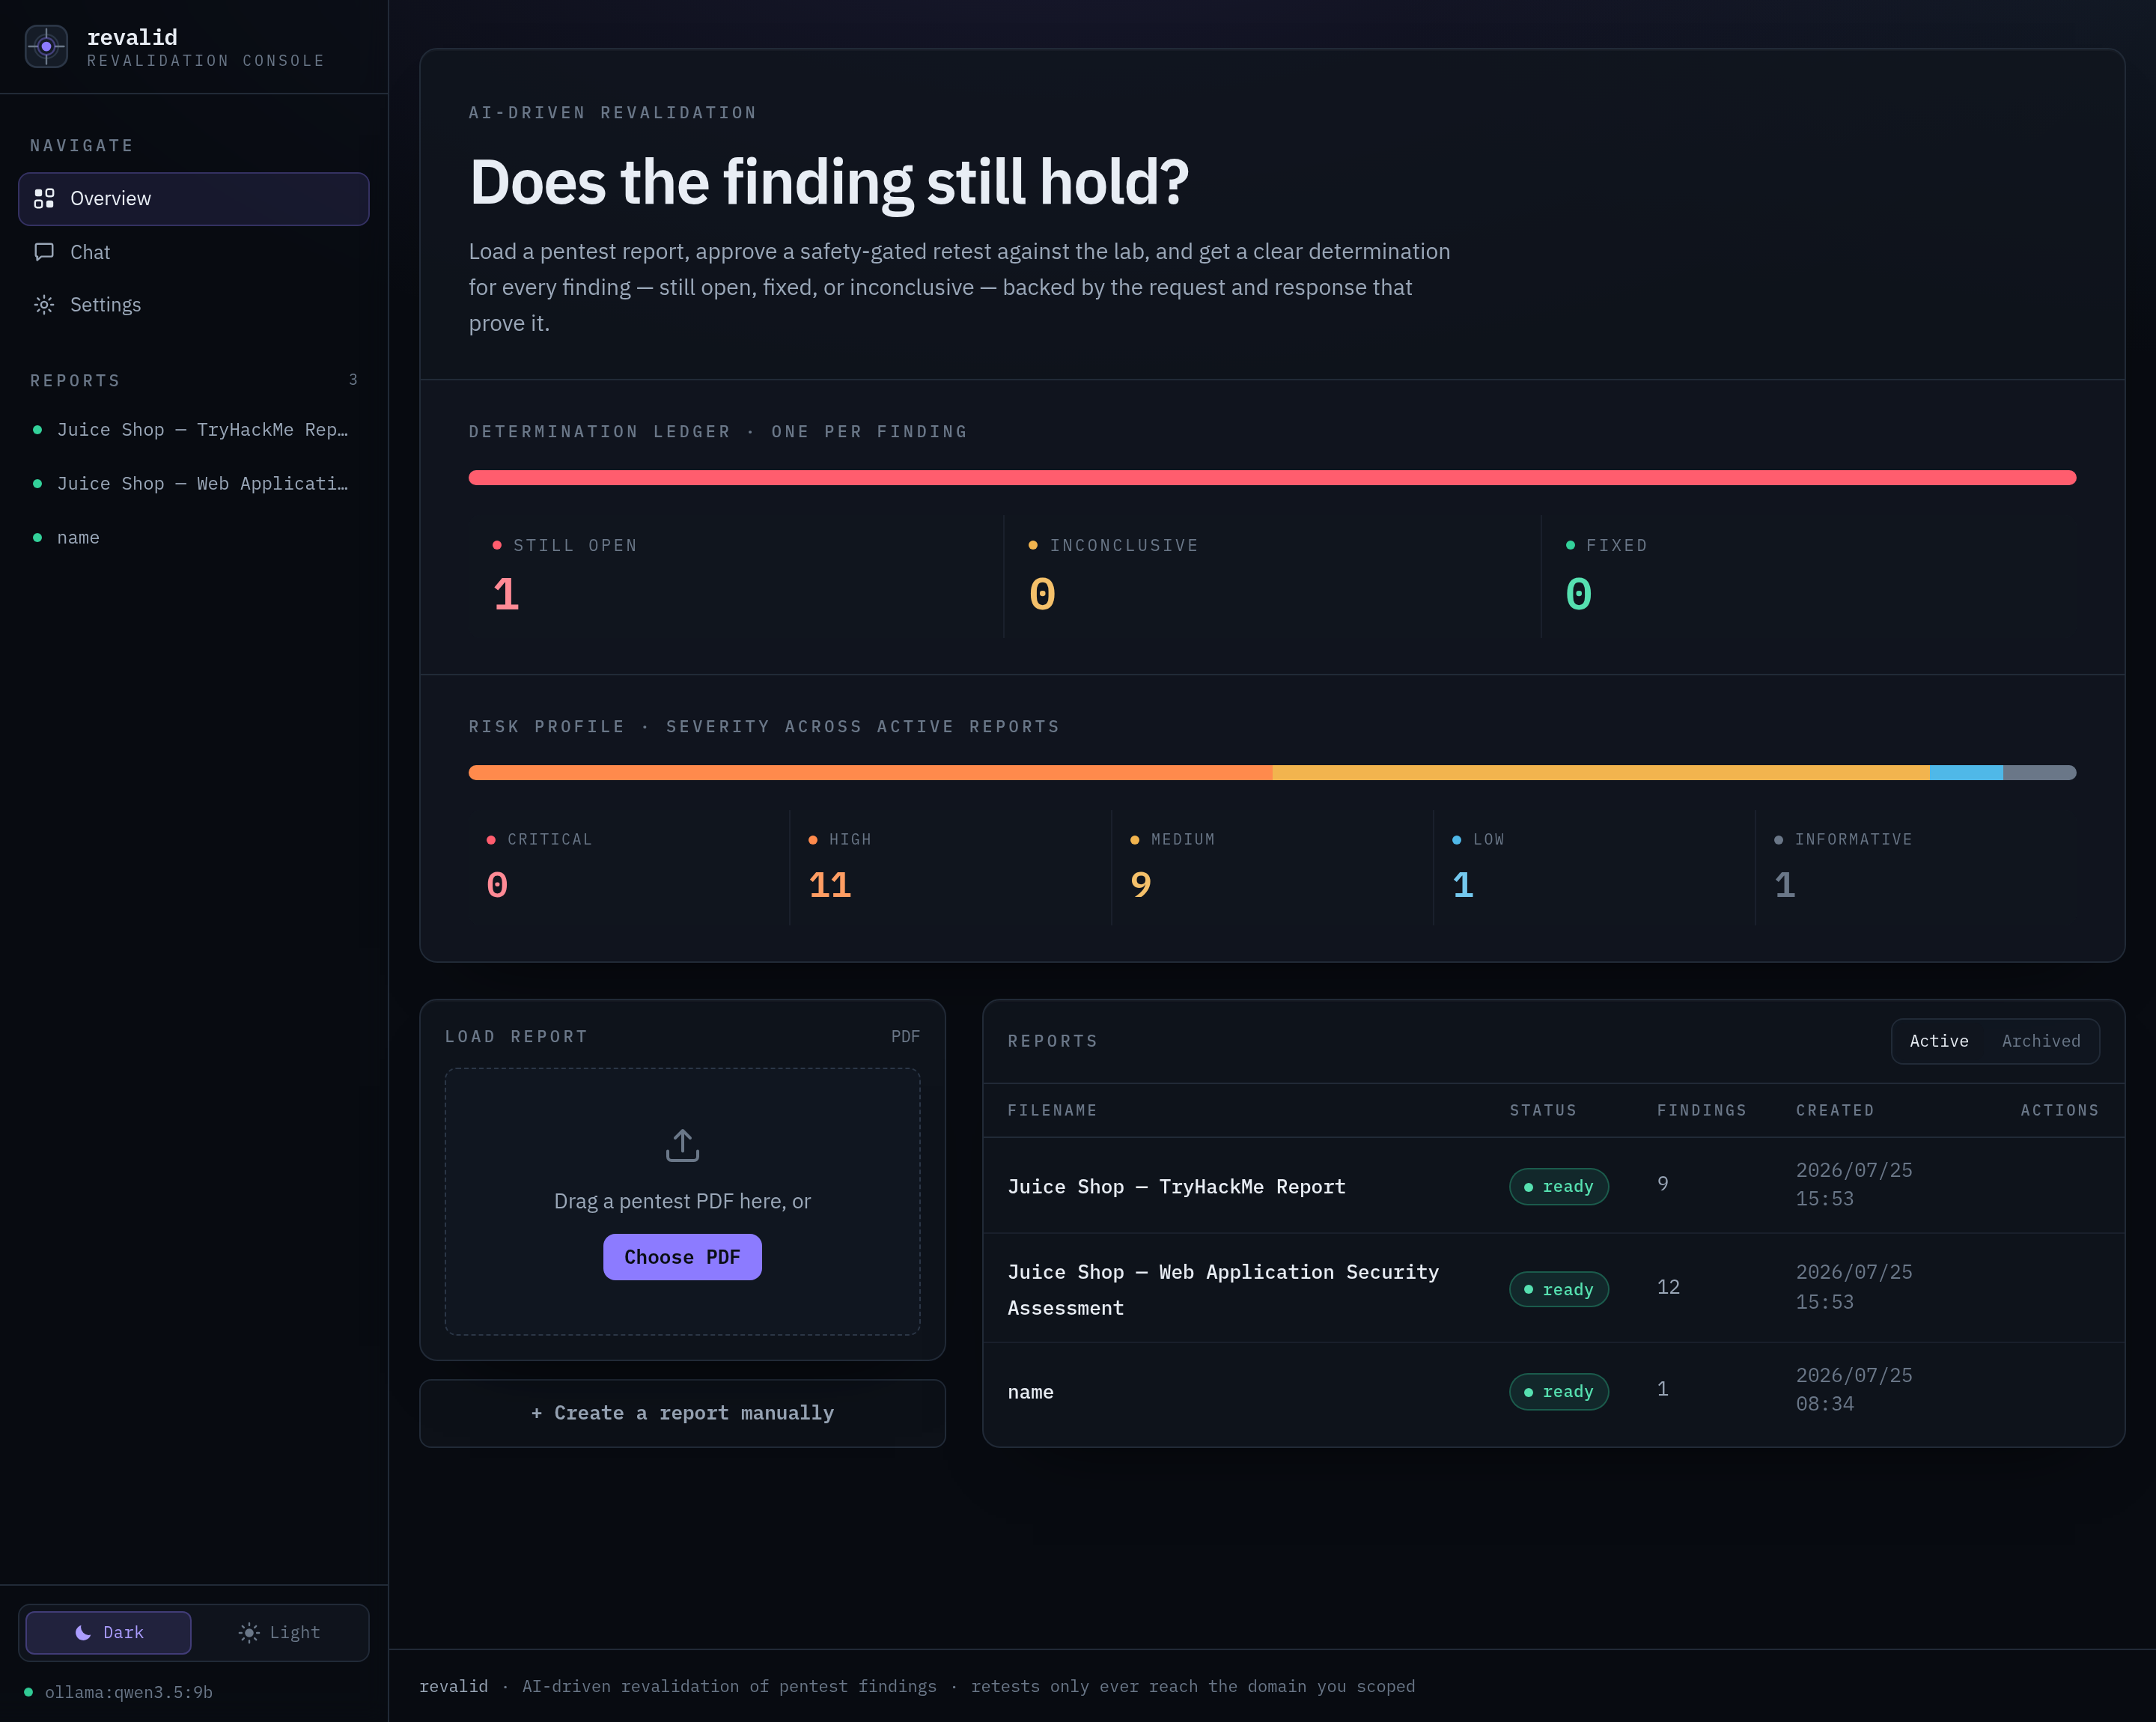
\includegraphics[width=\dimexpr\textwidth-2\fboxsep-2\fboxrule\relax]{figs/ui-overview.png}}
\caption[The overview]{The overview. One determination per finding (here none yet),
the severity profile across the loaded reports, and the report list. The two reports
are the evaluation inputs of Chapter~\ref{ch:evaluation}, loaded through the manual
door.}
\label{fig:ui-overview}
\end{figure}

Figure~\ref{fig:ui-console-gate} is the heart of the tool and of its safety claim:
the retest console with the agent \emph{suspended} on a proposed command. The command
and its one-line rationale are shown, the run cannot continue, and the only way
forward is the operator's \emph{Approve} or \emph{Reject}. The scope the session is
locked to is stated above; \emph{Conclude} is always available, so the operator can
end the retest at any point rather than only when the agent offers to.

\begin{figure}[htbp]
\centering
\fbox{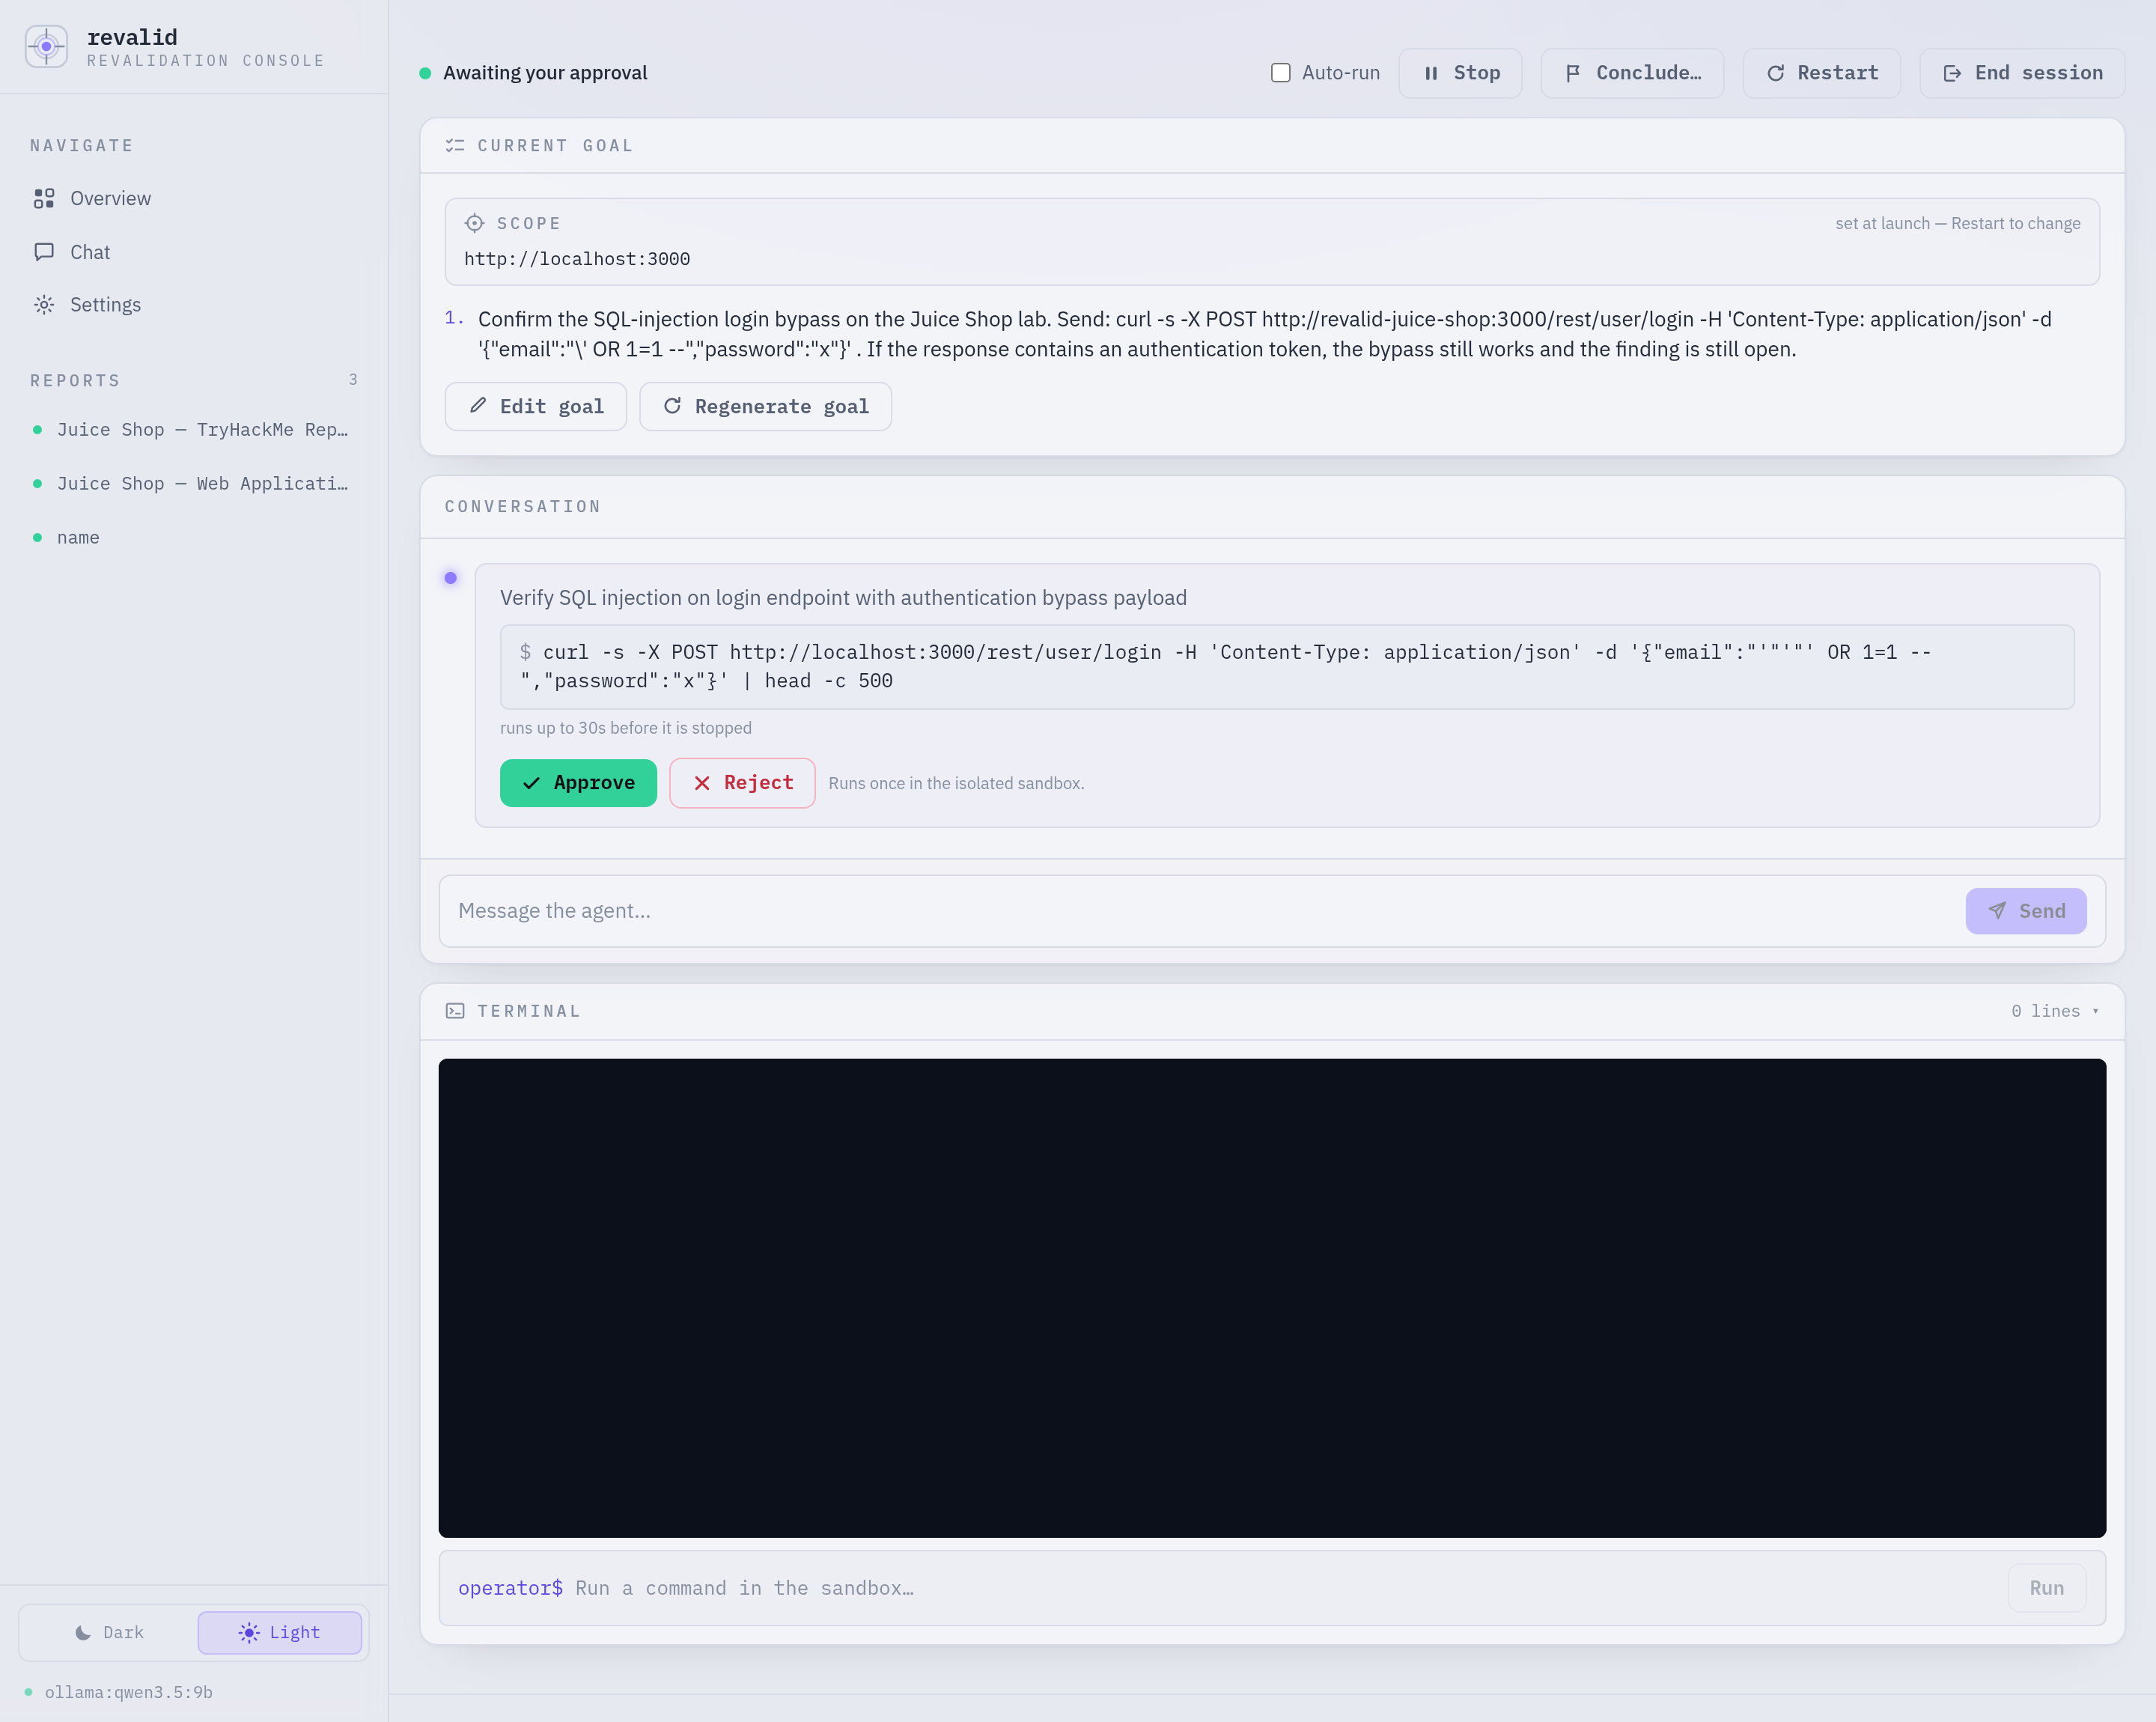
\includegraphics[width=\dimexpr\textwidth-2\fboxsep-2\fboxrule\relax]{figs/ui-console-gate.png}}
\caption[The approval gate]{The retest console at the per-command gate. The agent has
proposed a command to confirm the SQL-injection login bypass and \emph{suspended};
nothing reaches the target until the operator approves. This is the interaction the
whole design exists to enforce (FR-05, FR-17).}
\label{fig:ui-console-gate}
\end{figure}

Figure~\ref{fig:ui-console-terminal} shows what an approved command returns: the
console's terminal holds the \emph{real} captured output, here the administrator
session token the Juice Shop login-bypass yields, which is the evidence a
\emph{still-open} verdict is derived from. The two \texttt{operator\$} lines are the
operator running a command directly (ADR-0026) rather than approving one the agent
proposed --- one route among several the console offers, used here to address the
target by its in-sandbox container name.

\begin{figure}[htbp]
\centering
\fbox{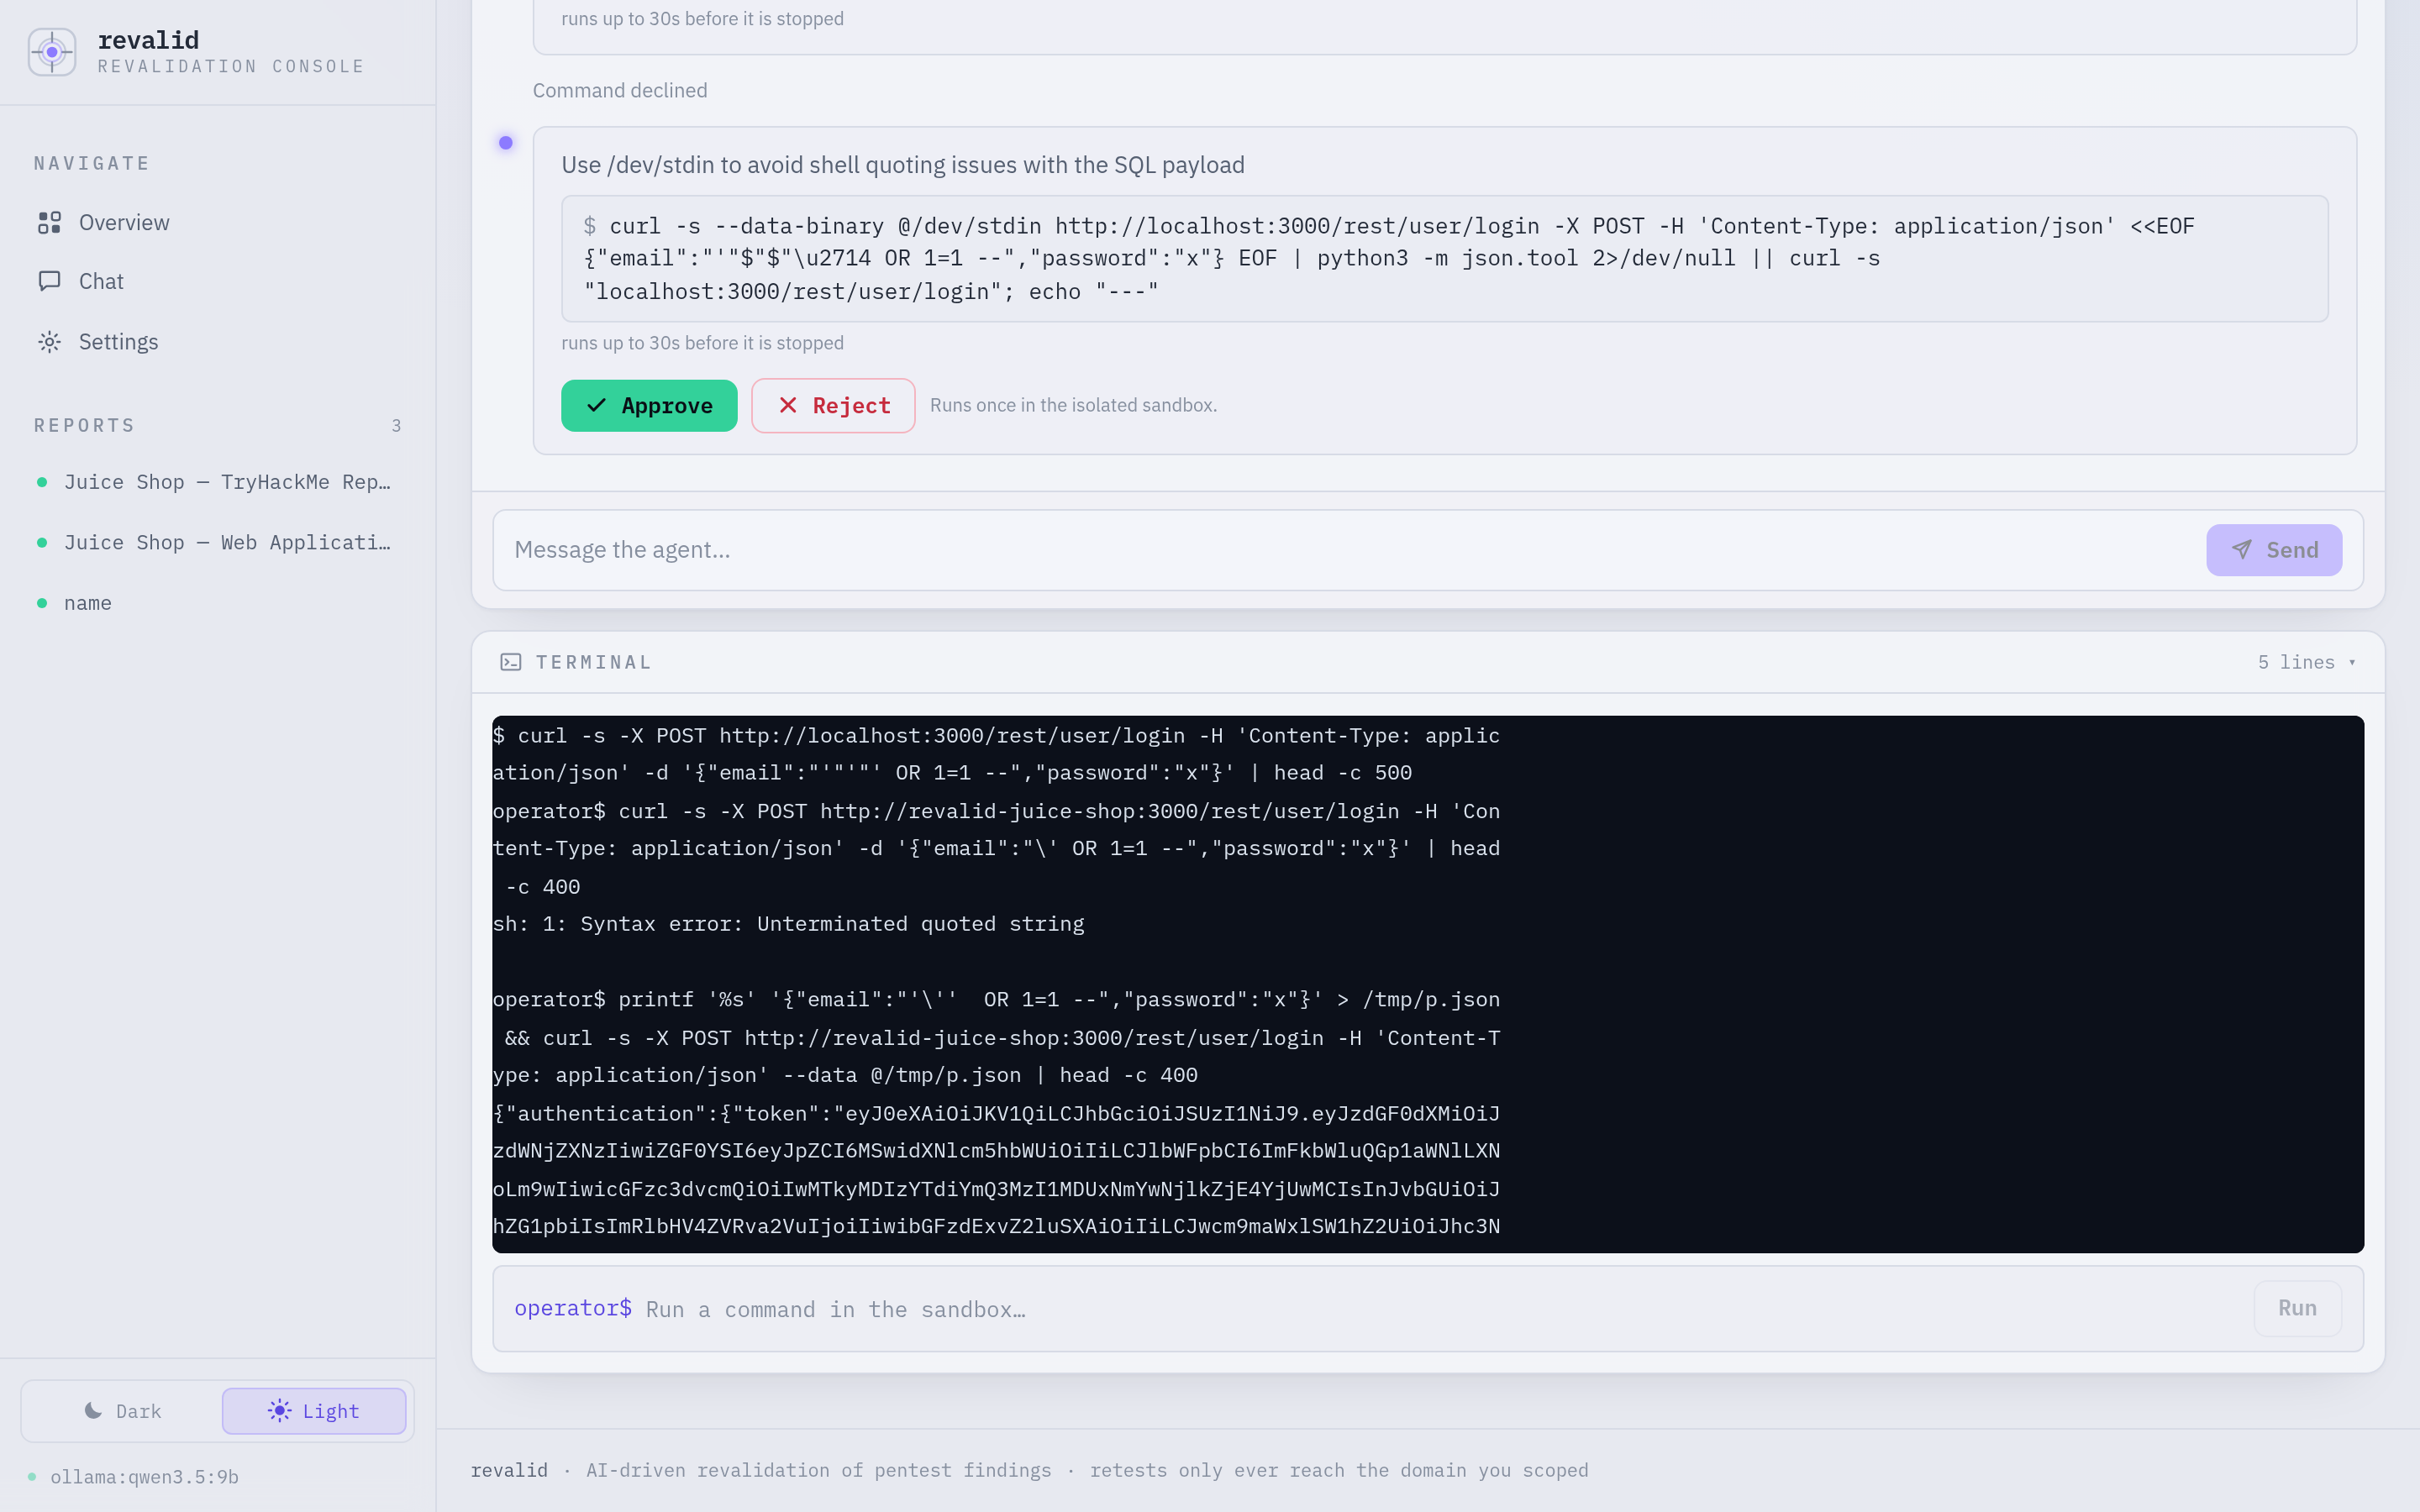
\includegraphics[width=\dimexpr\textwidth-2\fboxsep-2\fboxrule\relax]{figs/ui-console-terminal.png}}
\caption[Captured evidence]{The console terminal after execution. The response
carries a valid administrator authentication token, captured verbatim inside the
sandbox --- the evidence a verdict is pinned to, not the agent's recollection of it.}
\label{fig:ui-console-terminal}
\end{figure}

Figure~\ref{fig:ui-settings} shows the settings view, where the language-model
backend is chosen at runtime: a local Ollama server, a hosted Claude model or an
OpenAI-compatible endpoint, with the discovered models listed. This is the
model-agnostic layer of the design (FR-13) as the operator sees it, and it is what
makes the local-versus-hosted comparison of Chapter~\ref{ch:evaluation} a
configuration change rather than a rebuild.

\begin{figure}[htbp]
\centering
\fbox{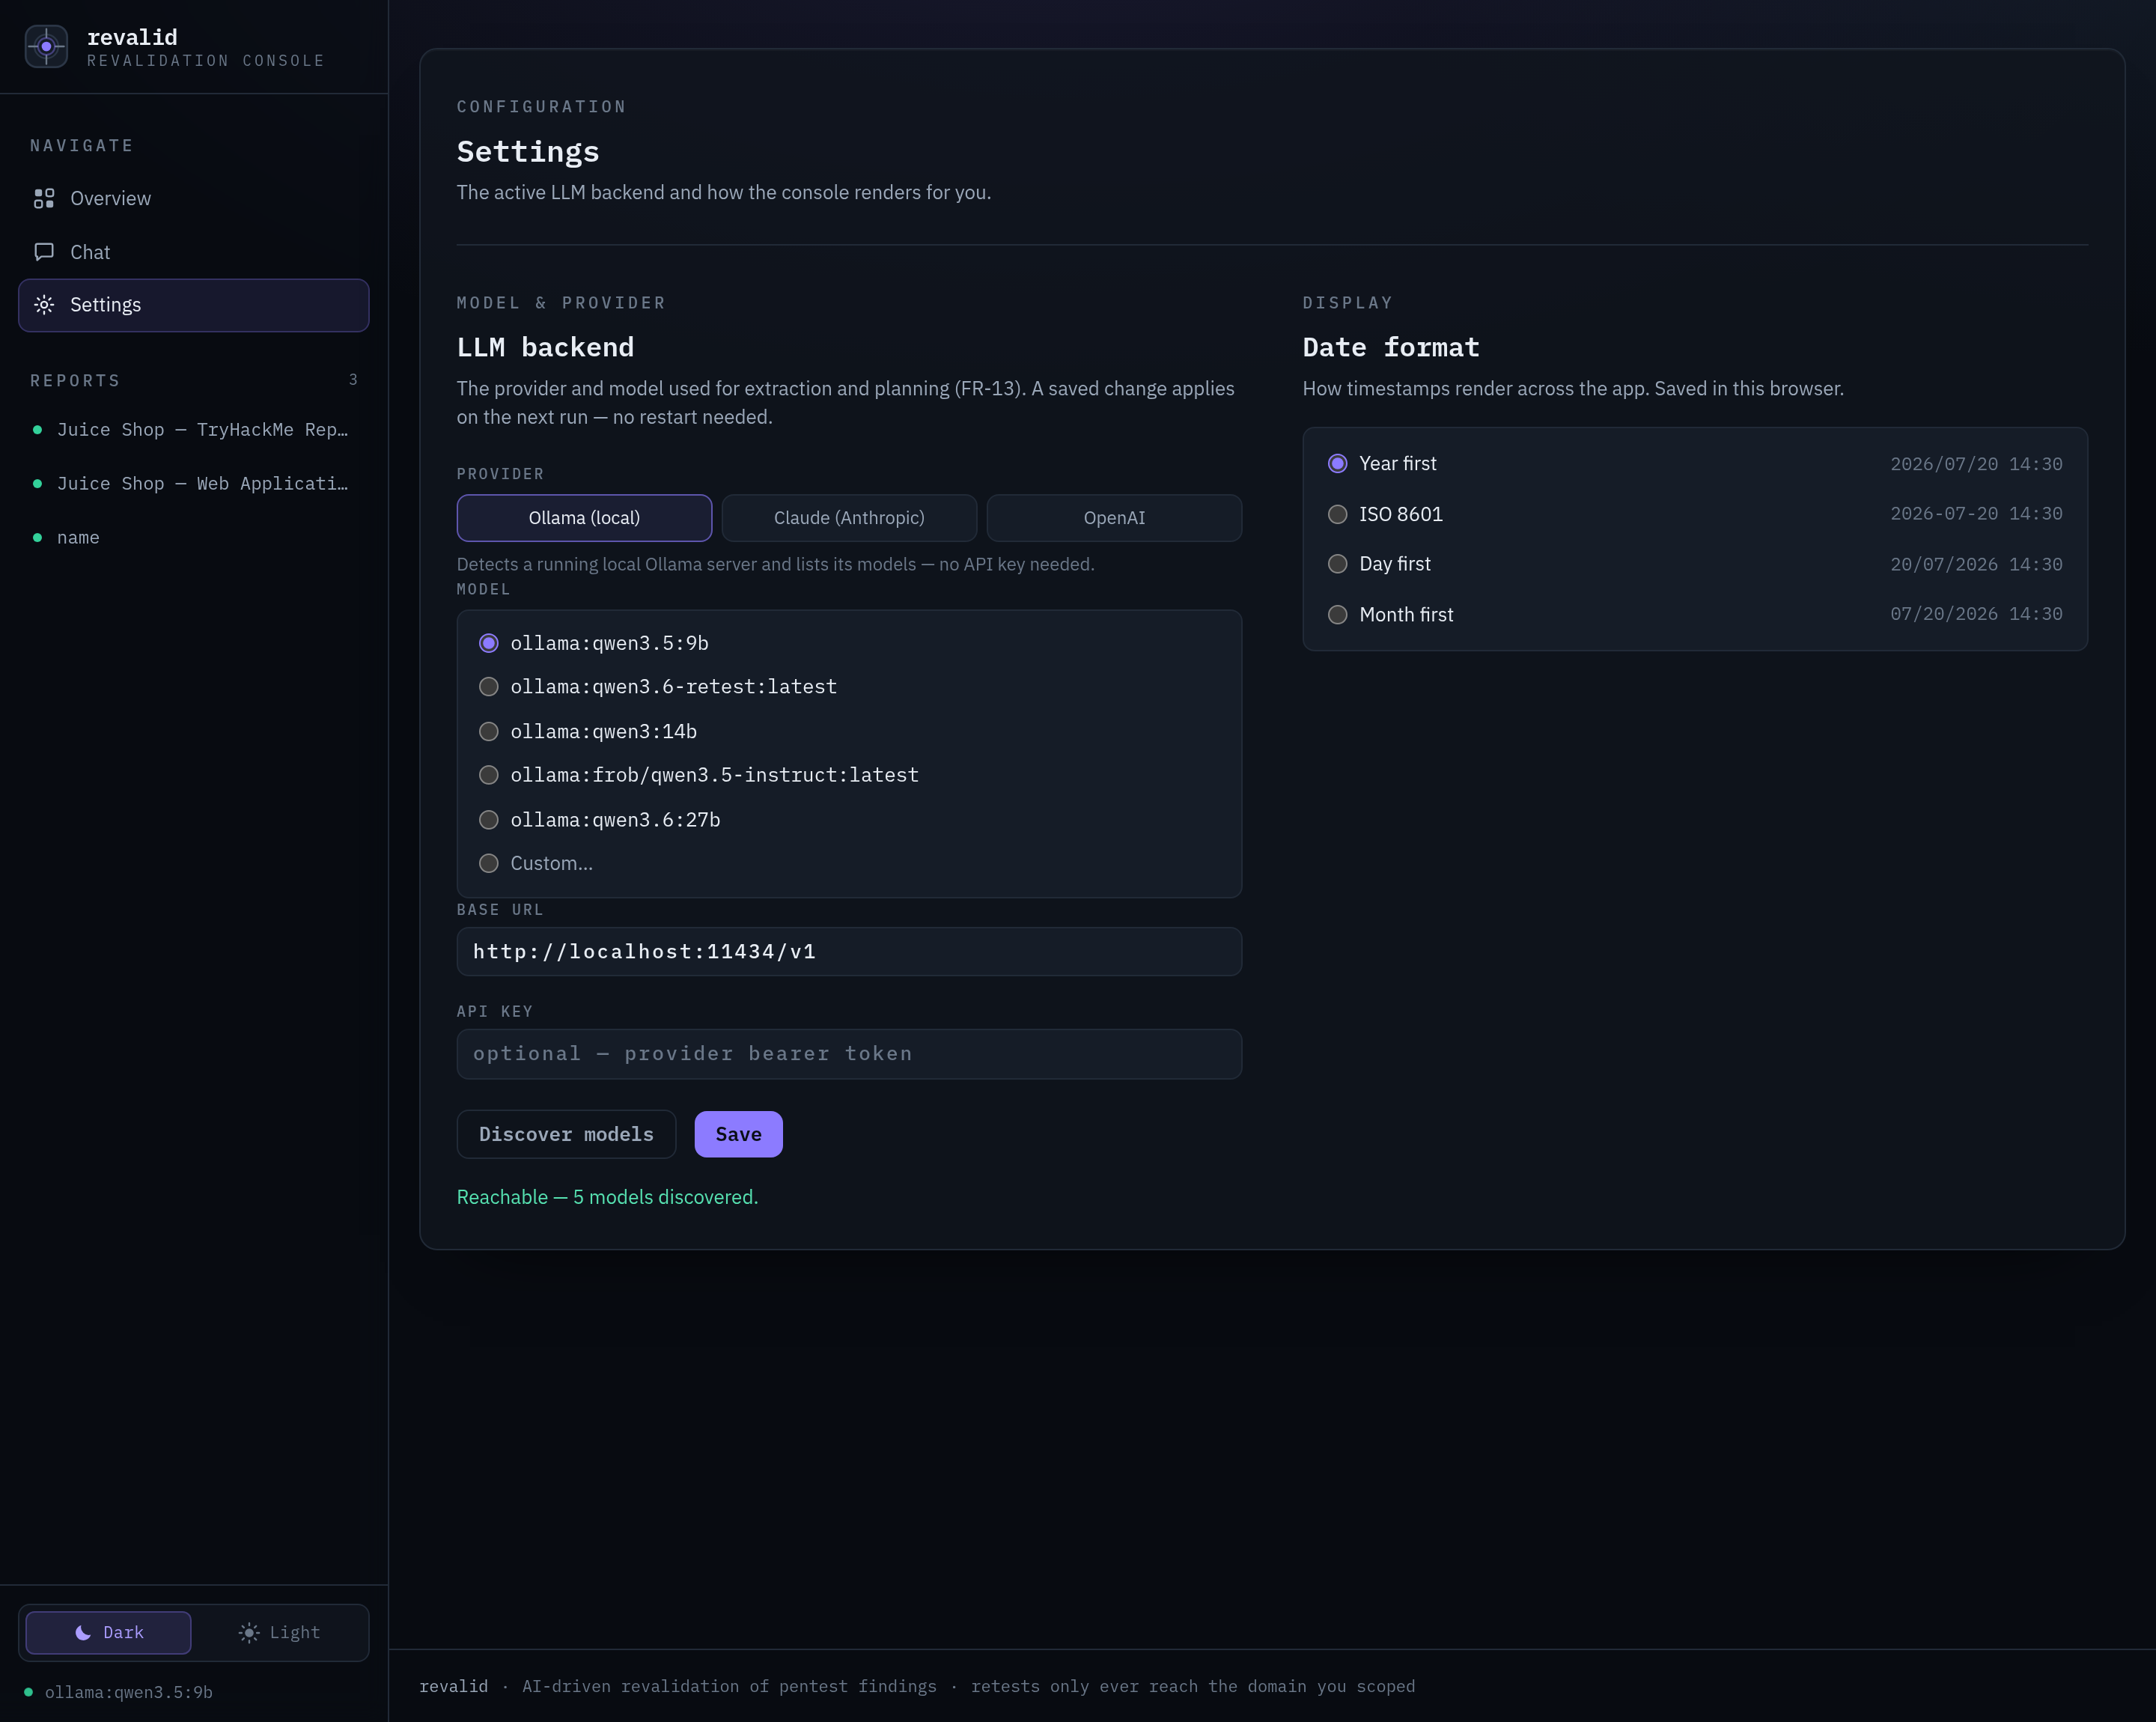
\includegraphics[width=\dimexpr\textwidth-2\fboxsep-2\fboxrule\relax]{figs/ui-settings.png}}
\caption[Choosing the backend]{The settings view. The provider and model are chosen
at runtime and take effect on the next run without a restart (FR-13); here a local
Ollama server is selected and its models discovered.}
\label{fig:ui-settings}
\end{figure}

\section{Offline demonstrations}
\label{sec:annex-demos}

Each stage of the pipeline can also be exercised headlessly, without the browser,
which is how the individual requirements are demonstrated and verified:

\begin{lstlisting}[language=bash]
make demo-ingest-pdf      # FR-01  PDF parsing into finding candidates
make demo-extract         # FR-03  language-model extraction
make demo-retest-session  # FR-17  gated agentic retest to a verdict
make demo-export          # FR-12  versioned run export
make demo-eval            # FR-15  evaluation harness over a run
\end{lstlisting}

Each runs without Docker, a lab target, a language-model backend or network access,
so all eight of them can be executed anywhere with \texttt{make test-demos}, which
is also what the continuous-integration gate runs on every change
(Section~\ref{sec:ci}).

\section{Resetting the state}
\label{sec:annex-reset}

All persistent state lives in a single local database file. It can be cleared to
start from a clean slate:

\begin{lstlisting}[language=bash]
make reset-db
\end{lstlisting}


\cleardoublepage
\thispagestyle{empty}


% -------------------------------
% Bibliografía
% -------------------------------
\bibliographystyle{apalike}
\bibliography{bib/ref}
\addcontentsline{toc}{chapter}{Bibliography}

\end{document}
